\graphicspath{{included-papers-tex/paper-9/}}

%\includedPaper{\textsc{paper vi - designer modeling through design style clustering}}{\textsc{paper vi - designer modeling through design style clustering}}{Alberto Alvarez, Jose Font, and Julian Togelius}

\includedPaper{\textsc{paper viii - Assessing the Effects of Interacting with MAP-Elites}}{\textsc{paper viii - Assessing the Effects of Interacting with MAP-Elites}}{Alberto Alvarez, Jose Font, Steve Dahlskog, and Julian Togelius}

\normalfont
\textbf{\textsc{ABSTRACT}}

MAP-Elites has been successfully applied to the generation of game content and robot behaviors. However, its behavior and performance when interacted with in co-creative systems is underexplored. This paper analyzes the implications of synthetic interaction for the stability and adaptability of MAP-Elites in such scenarios. We use pre-recorded human-made level design sessions with the Interactive Constrained MAP-Elites (IC MAP-Elites). To analyze the effect of each edition step in the search space over time using different feature dimensions, we introduce Temporal Expressive Range Analysis (TERA). With TERAs, MAP-Elites is assessed in terms of its adaptability and stability to generate diverse and high-performing individuals. Our results show that interactivity, in the form of design edits and MAP-Elites adapting towards them, directs the search process to previously unexplored areas of the fitness landscape and points towards how this could improve and enrich the co-creative process with quality-diverse individuals.

\textbf{\textsc{PUBLISHED IN}}

The 17th AAAI Conference on Artificial Intelligence and Interactive Digital Entertainment (AIIDE), AAAI, 2021.

\section*{ASSESSING THE EFFECTS OF INTERACTING WITH MAP-ELITES}

\subsection{Introduction}

% \begin{itemize}
%     \item This paper is analyzing the output of IC MAP-Elites while modifying the room~\citepninth{p9alvarez2019empowering}.
%     \item new papers that we can use: \citepninth{p9risi2019procedural,Risi2020GameAI,gaier2019quality,urquhart2019quantifying,charity2020mech}
%     \item Principles of mixed-initiative user interfaces \citepninth{p9horvitz1999principles} \citepninth{p9amershi2019guidelines}
%     \item Kate Compton Grokloop \citepninth{p9ComptonPhD} \\
    
% \end{itemize}
    
\begin{figure*}[ht!]
\centerline{\includegraphics[width=\textwidth]{figures/design-processes/combined.png}}
\caption{Sequences of rooms used in the three scenarios, targeting (a) low leniency, (b) high linearity, (c) and high meso-pattern concentration respectively. The leftmost and rightmost rooms correspond to the start and end rooms in each sequence, while intermediate steps are shown in between, limited to eight due to space restrictions.}
\label{figs:roomsexperiments}
\end{figure*}

% \begin{figure}
%     \centering
%     \includegraphics{figures/design-processes/combined.png}
%     \caption{Caption}
%     \label{fig:my_label}
% \end{figure}

%Procedural Content Generation (PCG) and AI-human blended approaches are two of the most promising focus areas for future game research in AI \citepninth{p9Risi2020GameAI}. PCG has now moved on from generating specific game content to almost complete game worlds \citepninth{p9nomansky,aidungeon}, as well as procedural learning environments and better benchmarks for training learning agents~\citepninth{p9Risi2020-pcgGeneralityML}. Evolutionary Computation (EC) is one of the dominant techniques in PCG \citepninth{p9yannakakis2014panorama}. 
Mixed-initiative co-creativity (MI-CC) \citepninth{p9yannakakis2014micc}, is a human-AI collaborative approach where both human and computer have a proactive role in the creation of content~\citepninth{p9liapis_generating_2013}. %shaker2013ropossum,
Recent research shows the importance of using quality-diversity (QD) algorithms \citepninth{p9Pugh2016,p9gravina2019procedural} to better drive the evolutionary process in complex search spaces by generating stepping stones that barely resemble the optimal solution \citepninth{p9gaier2019quality}. A popular QD implementation in recent research is MAP-Elites \citepninth{p9Mouret2015}, which has been applied to generate levels for bullet hell games \citepninth{p9Khalifa2018}, dungeon levels for MI-CC generation of adventure games~\citepninth{p9alvarez2019empowering}, and levels for puzzle games~\citepninth{p9charity2020baba}.% and mechanic-targeted level generation in Super Mario Bros \citepninth{p9Khalifa2019-intentionalCompLevel} and several games running on the GVG-AI framework \citepninth{p9charity2020mech}.  
% \begin{itemize}
%\item \citepninth{p9Khalifa2018} presented constrained MAP-Elites, a combination MAP-Elites with the feasible-infeasible concept from the FI2Pop genetic algorithm~\citepninth{p9Kimbrough2008}, and applied this to procedurally generating levels for bullet hell games. Another implementation of MAP-Elites has been recently used to produce small sections of Super Mario Bros levels called \textit{scenes}, addressing specific game mechanics \citepninth{p9Khalifa2019-intentionalCompLevel}.
% \item Mech-Elites: Illuminating the Mechanic Space of GVGAI \citepninth{p9charity2020mech} r introduces a fully automatic method of mechanic illumination for general video game level generation. Using the Constrained MAP-Elites algorithm and the GVG-AI framework
%\item  Quality Diversity (QD) algorithms are a better way to generate stepping stones than objective-based search \citepninth{p9gaier2019quality}
% \end{itemize}

%As the interest of the research community in PCG and MI-CC rises, so does the need for improving the ways for evaluating these novel approaches.
The rising interest of the evolutionary computation and computational intelligence in games research community in PCG, MI-CC and MAP-Elites, %drives the need 
calls for improving the ways for evaluating these novel approaches. Some of the main problems in mixed-initiative tools are the inadequate consideration of the costs and benefits for every automated action, as well as failing to spot the opportunities for users to guide the invocation of the automated services \citepninth{p9Horvitz99-mixedInit}. 
% Moreover, two of the design guidelines for AI-human interaction presented in \citepninth{p9amershi2019guidelines} address the need for facilitating users ways to edit and refine the AI system, and clearly communicating them why this system behaves as it does.
%The area of eXplainable AI for Designers (XAID) \citepninth{p9Zhu2018-XAIDesignersMICC} strives for %highlights the importance of 
%achieving system explainability %and concludes that this is 
%necessarily built on \textit{understandings of both algorithmic properties of the underlying AI techniques and the needs of human designers}. Similarly, Compton reflects on the so-called grokloop \citepninth{p9ComptonPhD}: the creative feedback MI-CC loop where a user builds a hypothesis, modifies a system, evaluates the result, and then updates the system. Shorter grokloops improve the overall performance of the mutual inspiration, and attempting to shorten this loop implies a clear understanding and interpretation of the relationship between each user action and the changes that it triggers in the system.

The area of eXplainable AI for Designers (XAID) \citepninth{p9Zhu2018-XAIDesignersMICC} strives for achieving system explainability necessarily built on \textit{understandings of both algorithmic properties of the underlying AI techniques and the needs of human designers}. Similarly, Compton reflects on the grokloop \citepninth{p9ComptonPhD}: the creative feedback MI-CC loop where a user builds a hypothesis, modifies a system, evaluates the result, and then updates the system. Shorter grokloops improve the overall performance of the mutual inspiration, and attempting to shorten this loop implies a clear understanding and interpretation of the relationship between each user action and the changes that it triggers in the system.
% Outside games, interactive use of algorithms 

% The area of eXplainable AI for designers (XAID) \citepninth{p9Zhu2018-XAIDesignersMICC} %is an umbrella term for all research works aiding game designers to utilize AI in their design tasks through co-creation. This work 
% highlights the importance of achieving system explainability, and concludes that this is necessarily built on \textit{understandings of both algorithmic properties of the underlying AI techniques and the needs of human designers}. Similarly, Compton reflects on the so-called grokloop \citepninth{p9ComptonPhD}: the creative feedback MI-CC loop where a user builds an hypothesis, modifies a system, evaluates the result, and then updates the system. Shorter grokloops improve the overall performance of the mutual inspiration, and attempting to shorten this loop implies clear understanding and interpretation of the relationship between each user action and the changes that it triggers in the system. 

% This study further evaluates the Interactive Constrained MAP-Elites, a continuous evolutionary process that takes advantage of MAP-Elites to provide QD procedurally generated dungeons, introduced in~\citepninth{p9alvarez2019empowering}. This explores the effects of continuous evolution and dimensions customization in an MI-CC approach. An in-depth analysis on the algorithm's expressive range of all feature-dimension pairs was presented in~\citepninth{p9Alvarez2020-ICMAPE} as the first step towards understanding how the generated solutions relate to all the dimensions included in the search space. 

%OLD
%In this paper we explore, analyze and discuss the dynamics of QD algorithms using the Interactive Constrained MAP-Elites in the domain of level generation of 2D adventure games. Through this we explore how IC MAP-Elites responds, reacts, and adapts to the editions and changes done by a designer in a mixed-initiative loop. We present results of the stability of the algorithm while constantly exploring for high-performing solutions in the generative space. Results also show that the interactive designer-algorithm loop opens up areas for exploration that previously seemed mutually exclusive regions of the search space.
%Shorter

MAP-Elites have shown excellent results at generating QD individuals in games~\citepninth{p9fontaine2019covariance,p9Alvarez2020-ICMAPE}, and offline adaptation based on its generated repertoire~\citepninth{p9Cully2015-qdRobotsAnimals,p9Gonzalez-Duque2020-DifficultyTrialError}. However, MAP-Elites generation capabilities have been mostly evaluated in non-interactive scenarios and based on its final result even when used in interactive situations~\citepninth{p9charity2020baba,p9alvarez2019empowering}. This results in a lack of research to assess the effects and consequences of interacting with MAP-Elites, and the adaptability and stability properties of MAP-Elites in dynamic scenarios. 

%MAP-Elites have shown excellent results at generating QD individuals in several areas such as games~\citepninth{p9fontaine2019covariance,Alvarez2020-ICMAPE} and robotics~\citepninth{p9nordmoen2020-MAPElitesStepStonesRobotics,Cully2019-QDAutonomousSkillDiscovery}, and offline adaptation based on its generated repertoire~\citepninth{p9Cully2015-qdRobotsAnimals,Gonzalez-Duque2020-DifficultyTrialError}. However, MAP-Elites generation capabilities have been mostly evaluated in non-interactive scenarios and based on its final result even when used in interactive situations~\citepninth{p9charity2020baba,alvarez2019empowering}. This results in a lack of research to assess the effects and consequences of interacting with MAP-Elites for both user and algorithm and the adaptability and stability properties of MAP-Elites in dynamic and interactive scenarios. 

% This hinders MAP-Elites' evaluation 

% Previous results 

% Previous results on \textit{"static"} evaluations for MAP-Elites suggests that both, the range of individuals generated and their performance, will be higher than other algorithms~\citepninth{p9cvt-mape2016,cully2020-multiemitter,Gravina2019-blendingNotionsDiversity}. However, the effects of this interactive loop and "dialogue" between user and algorithm, the continuous development, and ... is unknown. MAP-Elites have been used in interactive situations before~\citepninth{p9alvarez2019empowering,charity2020baba} and even used for modeling preferences and adapting its evaluation based on that with positive results~\citepninth{p9Alvarez2020-DesignerPreference}. Nevertheless, studies focus on evaluating MAP-Elites on static scenarios without any human interaction. Therefore, this paper aims at analyzing how interaction improves the evolutionary process and the mixed-initiative creative process in MAP-Elites.

% it has not been evaluated on the interactive system rather it has always been evaluated in a static scenario and on its own. Thus, we seek to answer is there any benefit for MAP-Elites and the user for using MAP-Elites in an interactive system?

% While MAP-Elites have shown excellent results for the generation of high-performing and diverse individuals in games~\citepninth{p9fontaine2019covariance}, robotics~\citepninth{p9Cully2015-qdRobotsAnimals}, and other areas, and have highlighted the benefits from its generated repertoire for more than creating diverse individuals, but also to allow rapid adaptation~\citepninth{p9Cully2015-qdRobotsAnimals,Gonzalez-Duque2020-DifficultyTrialError}
% For instance, imagine the scenario where an user is designing a robot piece by piece or some 3d objective?= in a CAD software that uses some type of recommendation, suggestions, assistance, or some type of mixed-initiative system. If we use an evolutionary algorithm for this assistance system, we will be able to explore the space vastly based on some type of objective, which if using \textit{interactive evolution} can be adaptive and provided by the user. Now, if we use MAP-Elites, based on previous results on \textit{"static"} evaluations, it can be estimated that both the range of individuals generated and their performance will be higher than other algorithms~\citepninth{p9cvt-mape2016,cully2020-multiemitter,Gravina2019-blendingNotionsDiversity}. However, the effects of this interactive loop and "dialogue" between user and algorithm, the continuous development, and ... is unknown. MAP-Elites have been used in interactive situations before~\citepninth{p9alvarez2019empowering,charity2020baba} and even used for modeling preferences and adapting its evaluation based on that~\citepninth{p9Alvarez2020-DesignerPreference} with good performance and positive results. Yet, it has not been evaluated on the interactive system rather it has always been evaluated in a static scenario and on its own. Thus, we seek to answer is there any benefit for MAP-Elites and the user for using MAP-Elites in an interactive system?


%This paper explores, analyzes, and discusses how population dynamics %in MAP-Elites 
%react and adapt to constant changes in the %Interactive Constrained MAP-Elites
%IC MAP-Elites for level generation of 2D adventure games. IC MAP-Elites is evaluated using simulated pre-recorded design sessions with different design goals that displays the algorithm's stability and adaptability properties, and benefits. We present results of the stability of the algorithm while constantly exploring high-performing solutions in the generative space. Results also show that the interactive designer-algorithm loop opens areas for exploration that previously seemed mutually exclusive regions of the search space.

Therefore, the contributions of this paper are two-fold. On the one hand, we present Temporal Expressive Range Analysis (TERA) as a novel way to analyze interactive PCG. TERAs allow us to inspect and analyze the changes in the expressive range over a defined period, which in our case, are design editions. On the other hand, using TERAs, we explored and analyzed how population dynamics react and adapt to constant changes in the IC MAP-Elites for level generation of 2D adventure games. IC MAP-Elites is evaluated using simulated pre-recorded design sessions with different design goals that display the algorithm's stability and adaptability properties and benefits. Our results show that IC MAP-Elites stably encounters high-performing solutions while adapting to changes in the design, and by doing this, regions of the search space which previously seemed inaccessible are opened for exploration.

% . We also show that the interactive designer-algorithm loop opens areas for exploration that previously seemed mutually exclusive regions of the search space.  

% This paper explores, analyzes, and discusses how population dynamics react and adapt to constant changes in the IC MAP-Elites for level generation of 2D adventure games. IC MAP-Elites is evaluated using simulated pre-recorded design sessions with different design goals. In order to evaluate the algorithm, we present Temporal Expressive Range Analysis (TERA) as a novel way to analyze interactive PCG. TERAs allow us to inspect and analyze the changes in the expressive range over a defined period, which in our case, are each design edition. 

% IC MAP-Elites is evaluated using simulated pre-recorded design sessions with different design goals. In order to evaluate and analyze the algorithm's stability and adaptability properties, we also present Temporal Expressive Range Analysis (TERA). TERAs allow us to inspect and analyze the changing expressive range 

% In order to  These are evaluated 


% that display the algorithm's stability and adaptability properties and benefits. We analyze We present results of the stability of the algorithm while constantly exploring high-performing solutions in the generative space. Results also show that the interactive designer-algorithm loop opens areas for exploration that previously seemed mutually exclusive regions of the search space. 
\subsection{Background}

%\subsubsection{The Evolutionary Dungeon Designer} 
%Summarize EDD in its current status (what's described on the IEEE TOG paper).

%\subsubsection{Evolving Dungeons as a Whole, Room by Room}

% \begin{figure}[t]
% \centerline{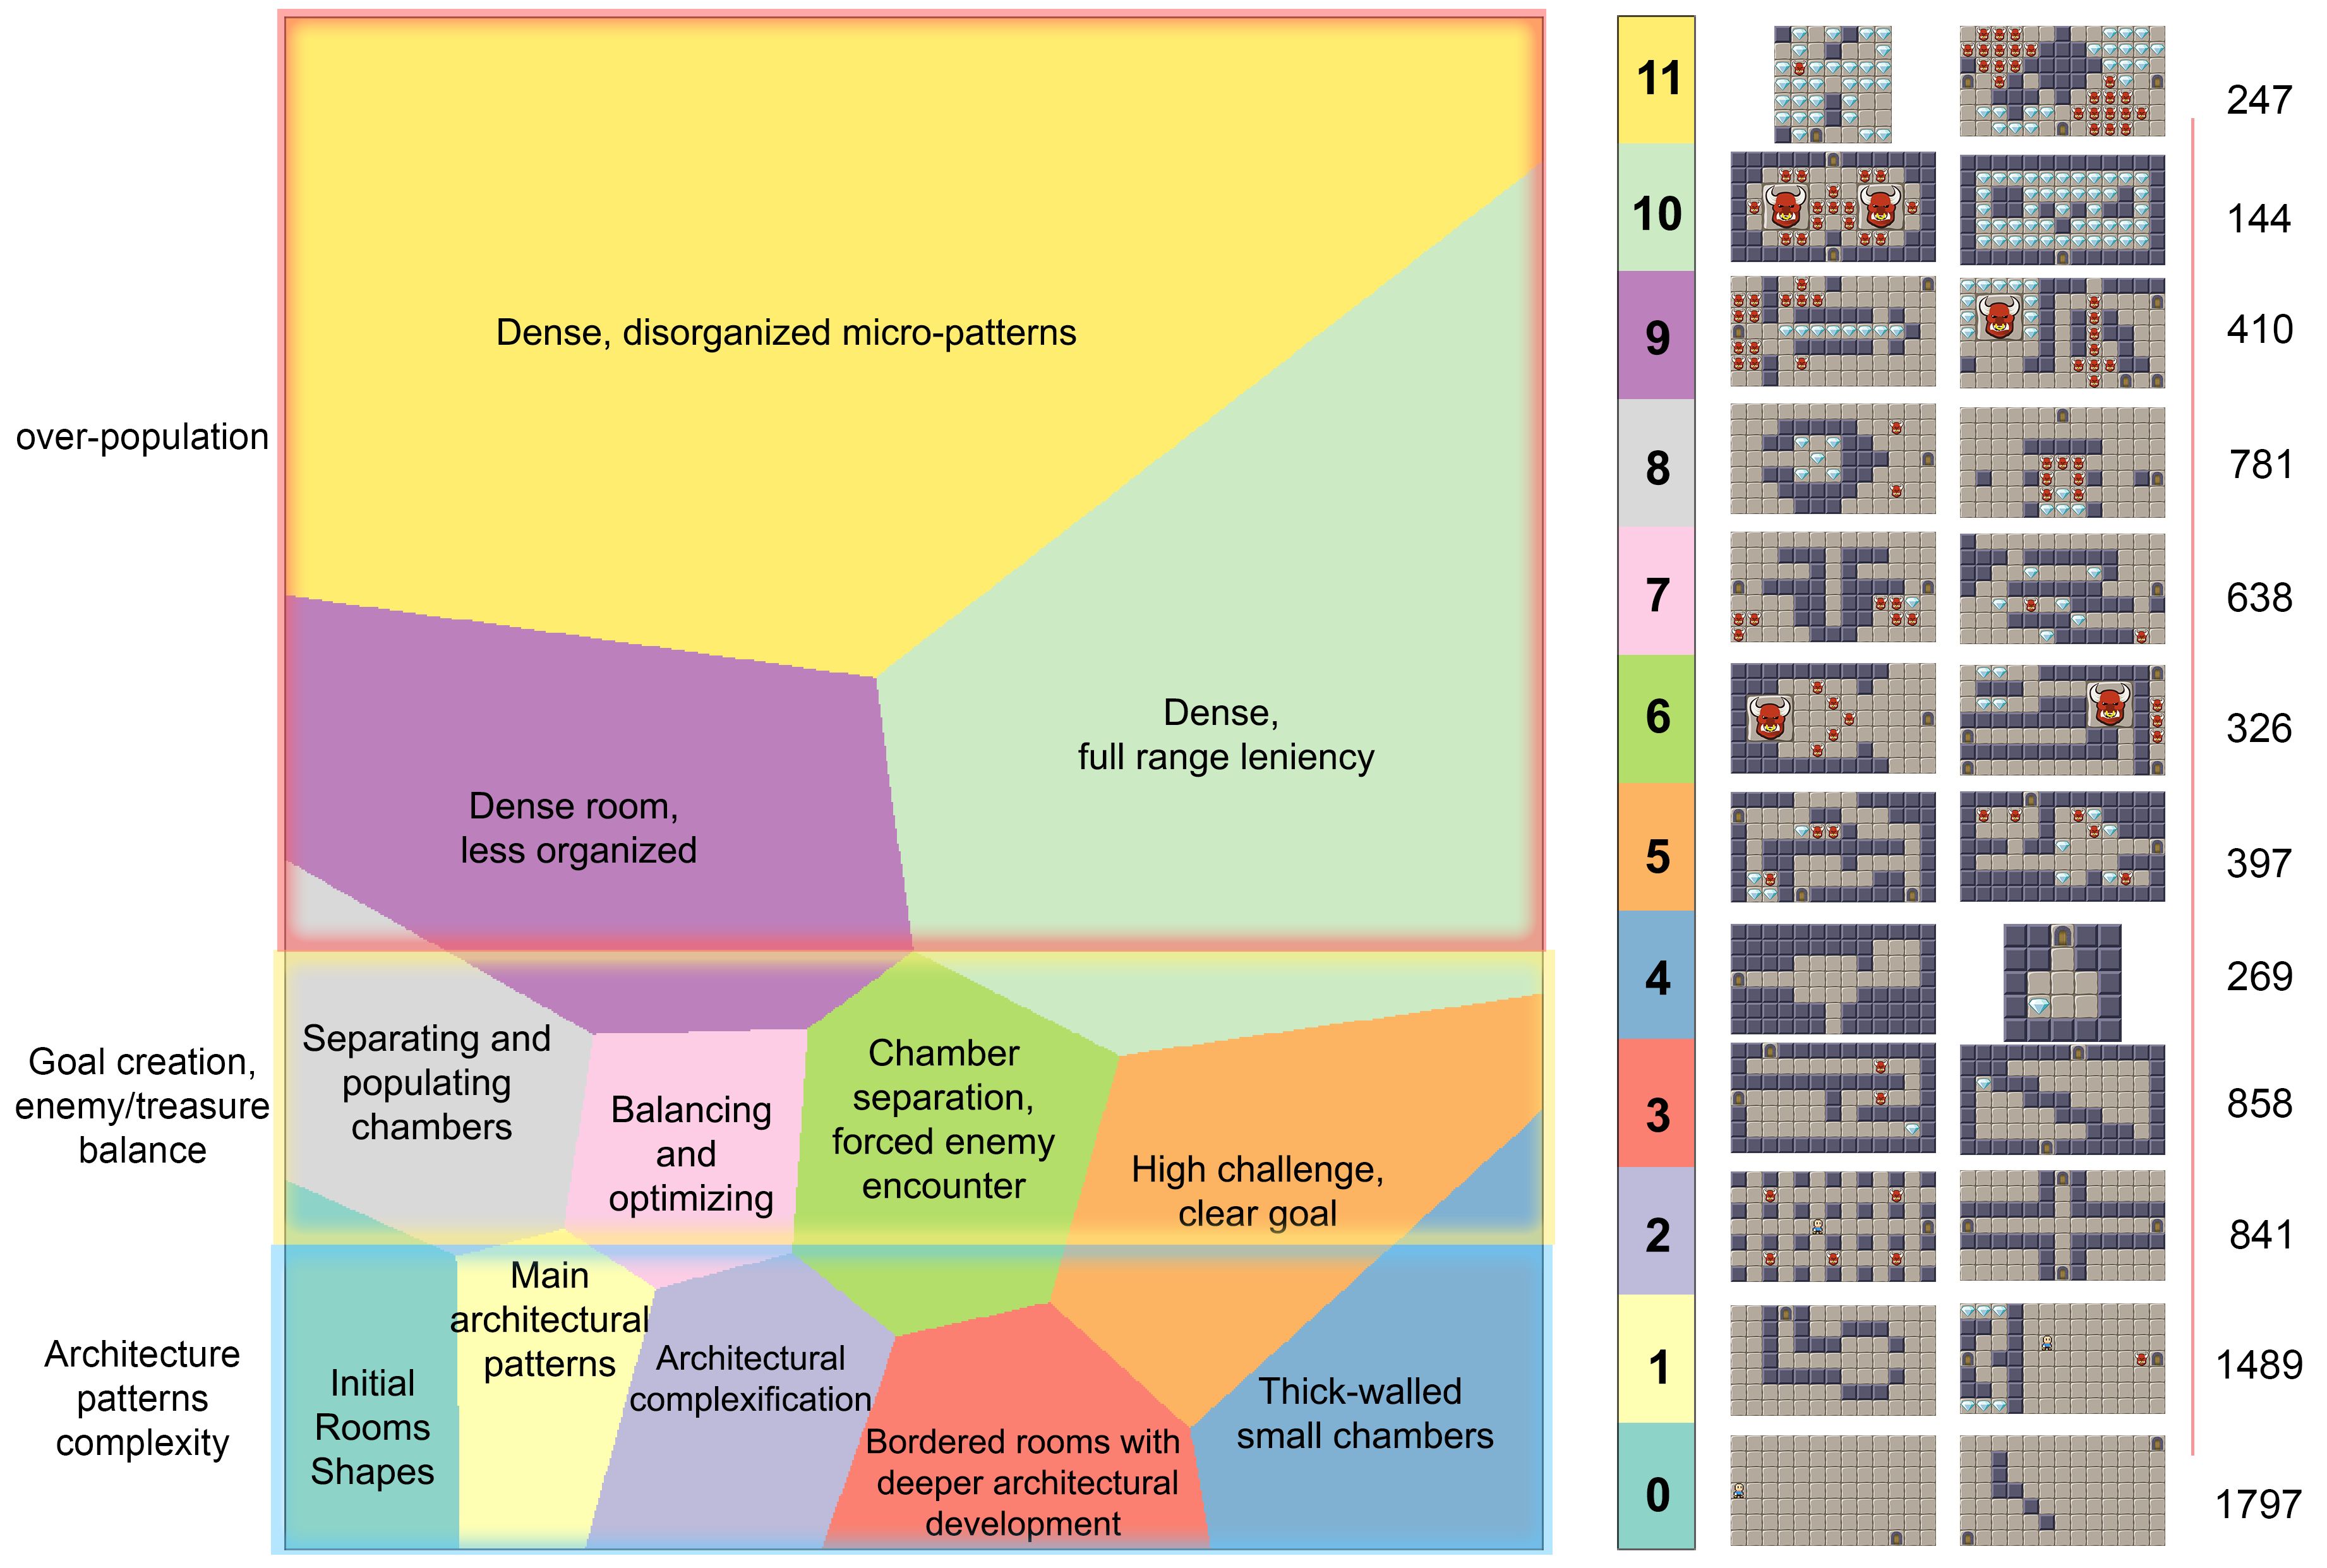
\includegraphics[width=9cm]{figures/figure2.png}}
% \caption{Screenshot of the dungeon editor screen in EDD, displaying a sample dungeon composed by seven rooms. The shortest path between two given tiles is highlighted in blue. The right pane contains all options for editing the dungeon. "M", "C", and "P" stand for "Move rooms", "Connect rooms", and "calculate Path".}
% \label{figs:dungeonscreen}
% \end{figure}
% \begin{figure}[t]
% \centerline{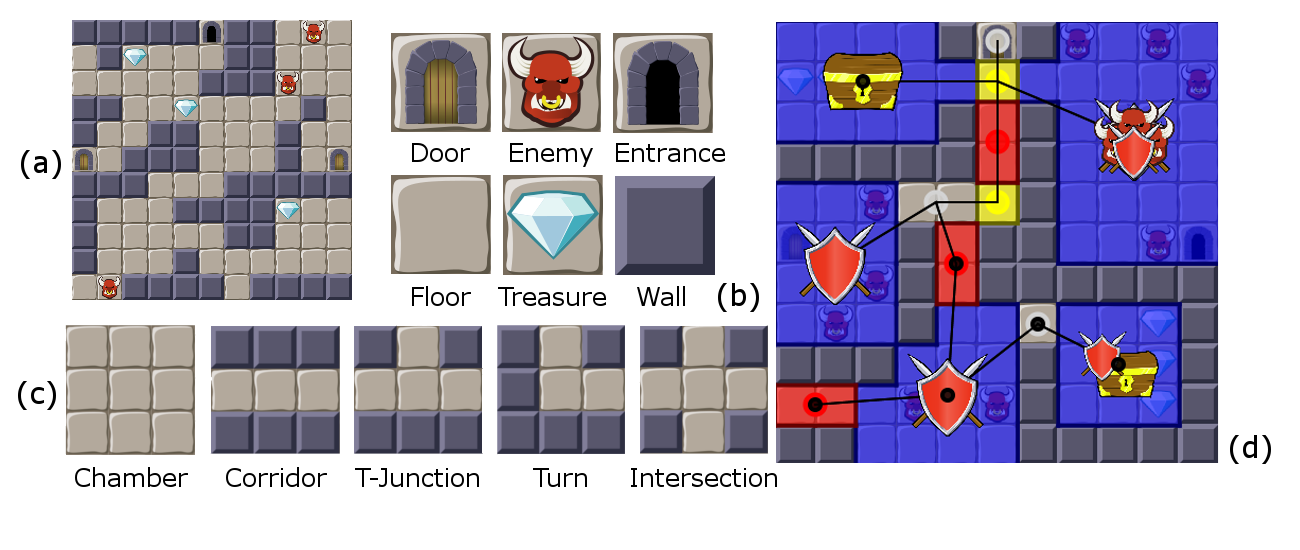
\includegraphics[width=9cm]{figures/figure1.png}}
% \caption{The EDD components. (a) A room, (b) placeable tiles, (c) micro- and (d) meso-patterns~\citepninth{p9Alvarez2018a}.}
% %\caption{The main components in EDD. (a) A basic room, (b) different placeable tiles, (c) micro-patterns and (d) meso-patterns~\citepninth{p9Alvarez2018a}.}
% \label{figs:basecomponents}
% \end{figure}


%The Evolutionary Dungeon Designer (EDD) is a Mixed-Initiative Co-Creativity (MI-CC) tool under continuous development. Its purpose is to allow a human designer create, or co-create with the AI, a 2D dungeon with rooms and corridors in the style of those appearing in the seminal game \emph{The Legend of Zelda}~\citepninth{p9tloz}.
The Evolutionary Dungeon Designer (EDD) is a MI-CC tool %under continuous development. It that allows 
to %create, or 
co-create 
%with the AI, 
2D dungeons in the style of the seminal game \emph{The Legend of Zelda}~\citepninth{p9tloz}.
%in the style of those appearing in the seminal game
% (\Cref{figs:basecomponents}.a).  The EDD workflow lets the 
Designers manually edit the dungeon structure as well as the interior of every room in it. EDD constantly offers tailored room suggestions on the fly that designers may decide to incorporate to their designs at any moment. 

In EDD, the system analyzes the level-design patterns (i.e., micro- and meso-patterns) that exist in each room, calculating and utilizing their quality to assess rooms. Micro-patterns are the building blocks in a design, which in EDD are categorized as \textit{spatial micro-patterns}: chamber, corridor, intersections, connector; and \textit{inventorial micro-patterns}: enemy, treasure, and door. On the other hand, Meso-patterns are defined as the relation between micro-patterns or other meso-patterns, and by the composition between inventorial micro-patterns and spatial micro-patterns. Meso-patterns are used to identify structures in the room that join together a set of micro-patterns and can be: \textit{ambush}, \textit{guard chamber}, \textit{treasure chamber}, and \textit{guarded treasure}. All patterns are shown in figure~\ref{fig:basecomponents}, and further information and discussion can be found in~\citepninth{p9Baldwin2017,p9Alvarez2018}.

\begin{figure}[b]
\centerline{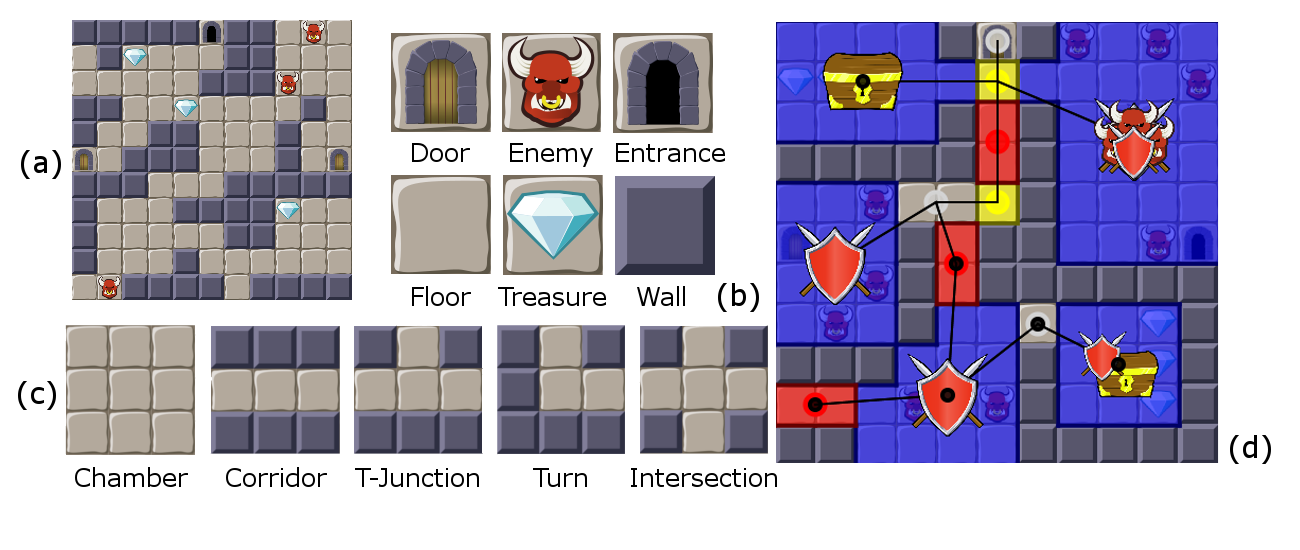
\includegraphics[width=9cm]{figures/figure1.png}}
\caption{Main components in EDD. (a) Basic room, (b) different tiles, (c) micro-patterns and (d) meso-patterns}
\label{fig:basecomponents}
\end{figure}


%to edit the dungeon by adding or removing rooms or by editing the rooms' tiles.
%The EDD workflow let the designer to manually edit the dungeon by adding or removing rooms or by editing the rooms' tiles.% (\Cref{figs:basecomponents}.b)  (\Cref{figs:basecomponents}.c and \Cref{figs:basecomponents}.d). A detailed description of all EDD's features, including the use of game design patterns, can be found in~\citepninth{p9Baldwin2017a, Baldwin2017, Alvarez2018, Alvarez2018a}. The foundation of the MI-CC approach in EDD is the use of EC aiming to find optimal candidates with game design patterns and design symmetry as objectives for the evolutionary search.

% An extensive description of EDD's features can be found throughout~\citepninth{p9Baldwin2017,Alvarez2018} %~\citepninth{p9Alvarez2018}

% as well as a complete description of its underlying %. The latest extension to EDD is the utilization of 
% IC MAP-Elites~\citepninth{p9Alvarez2020-ICMAPE}.
%With this function the designer can pick and choose from different procedurally generated room suggestions. With this function With this, the designer can choose from diverse room suggestions. The IC MAP-Elites are provided by continuous evolution and visually organized by dimensional customization.
%\begin{figure*}[t]
%\centerline{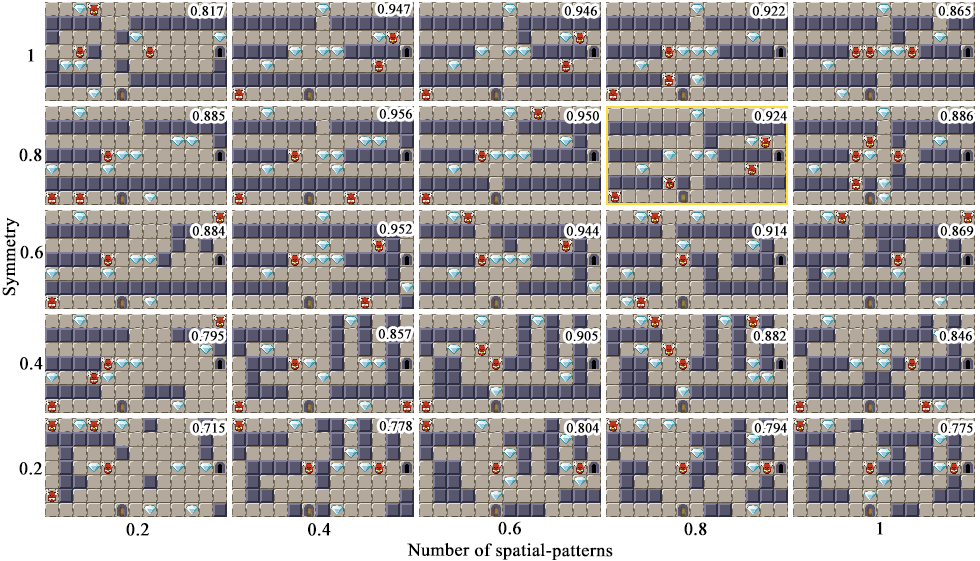
\includegraphics[width=13cm]{figures/figure3.jpg}}
%\caption{The room editor screen in EDD. The left pane contains all the options for manually editing the room displayed at the center-left of the screen. The right section displays the procedurally generated suggestions.}
%\label{figs:roomscreen}
%\end{figure*}
%In this section we present the latest version of EDD\footnote{Available for download at \url{https://github.com/mau-games/eddy}}, which includes significant improvements based on the outcomes from the qualitative analysis discussed in~\citepninth{p9Alvarez2018}. The most significant upgrade is replacing the grid-based backbone that represented the dungeon by a more flexible graph-based representation. A dungeon is now a graph of interconnected rooms of any given size between $3\times3$ and $20\times20$ tiles. The smallest allowed dungeon is composed by two rooms with one connection to each other. The designer can perform the following new actions: 
%\begin{itemize}
%\item adding disconnected rooms to the dungeon. Rooms may also be removed at any time.
%\item connecting any pair of rooms by adding a new bi-directional connection to the graph. Rooms interconnect from and to passable border tiles (self-loops are not allowed). Both ends are marked with a door tile (\Cref{figs:basecomponents}.b). A single border tile can only hold one connection, implying that a room can have as many connections as passable border tiles. Connections and rooms can be removed at any time, and their associated doors removed with them.% Removing a room also removes its connections.
%\item calculating paths between any pair of passable tiles located in any connected room. Paths are automatically calculated according to one of the following heuristics: \textit{fastest} returns the shortest path, \textit{rewarding} returns the path that traverses the highest number of treasure tiles, \textit{less danger} provides a path with the fewest number of enemies, whereas \textit{more danger} does the opposite. 
%\end{itemize}
%The designer is required to select one of the added rooms as the \textit{initial room}, which is the first room the player meets when entering the dungeon. This selection can be modified unlimited times. The \textit{initial room} is used by EDD to calculate the feasibility of the dungeon. A dungeon is considered feasible when there is at least one path between the \textit{initial room} and any other passable tile in every room. Rooms and doors that are unreachable from the \textit{initial room} are highlighted in red, so that they can be easily identified by the designer. This feasibility constraint ensures that all passable tiles are accessible, avoiding the possibility of accidentally creating unreachable areas.  
% \paragraph{The mixed-initiative workflow in EDD}
%The starting screen in EDD is the dungeon editor screen. Every new room is empty (composed solely of floor tiles) when created and is placed detached from the dungeon graph. After manually connecting the room to the dungeon with at least one connection, the designer has the option to populate the room using the room editor screen (\Cref{figs:roomscreen}). This screen can be reached in two different ways:

%\begin{enumerate}
%\item directly: by double-clicking or zooming in (by using the mouse wheel or by pinching on the touchpad) on the room. 
%\item indirectly: by clicking on the "Start with our suggestions" button, six procedurally generated suggestions are displayed on a separate screen. The selected suggestion is then opened in the room editor screen. 
%\end{enumerate}

%\Cref{figs:roomscreen} shows the room editor screen displaying a sample room with the dimensions $7\times5$ tiles. The left pane lists all the available options for manually editing the room. Manual editing is carried out by brush painting over the room with one of the available tile types: floor, wall, treasure, or enemy. There are two brush sizes (single tile and five-tile cross shape), and control-clicking allows the designer to bucket paint all adjacent tiles of the same type. Brush painting with the lock button on preserves selected tiles in all the procedurally generated suggestions. A detailed description of all the options in this pane is included in~\citepninth{p9Alvarez2018, Alvarez2018a}.

%The right side of the screen displays the procedurally generated suggestions, by means of the Interactive Constrained MAP-Elites genetic algorithm (see \Cref{section:3}).  
%When the designer accesses the room editor screen, the EA starts and continuously populates the suggestions pane with elites. The evolutionary process is fed with the manually edited room (i.e. target room), so that every change in the room affects the generated suggestions. By clicking on "Apply Suggestion", the manually edited room is replaced by the selected suggestion, thus affecting the upcoming procedural suggestions. "Restart" restarts the EA, and "Go To World Grid" takes the user back to the dungeon editor screen.

\subsubsection{Methods for Evaluating PCG}

%Over the last few years 
Recent research %In recent years a %small number of research initiatives have focused 
focuses on methods for evaluating procedural algorithms. The work in~\citepninth{p9Gravina2019-blendingNotionsDiversity} %the experimental set-up is a soft robots evolution task and covers:
evaluates fitness, offspring and selection for five MAP-elite methods, whereas %The results exhibit good effects by joining novelty and surprise in Quality Diverse (QD) algorithms. %The results demonstrates good effects by incorporating novelty and surprise in Quality Diverse (QD) algorithms. Another approach to optimise procedural generation has been explored by Cook et al.~\citepninth{p9Cook2016-SecondPaperDanesh} and Another approach to optimise procedural generation
\citepninth{p9Cook2016-SecondPaperDanesh} shows how users can improve the generator with the aid of automatic parameter tuning and, consequently, evaluates the effect that it has on the generator. The work is continued in~\citepninth{p9Cook2019:ParameterBasedEvaluation} where two analytical techniques, smoothness and co-dependence, were introduced to analyze the impact of a parameter change and its %following 
effect on a generative system; all integrated in Danesh~\citepninth{p9Cook2021-danesh}. Liapis et al.~\citepninth{p9Liapis2014-designerModelImpl} did a similar evaluation as the one in this paper, using artificial agents simulating designer's choices of suggestions to evaluate and display properties of their designer's model.%, in this case a cellular automata-based system. By doing so, it is possible to work with procedural generators more precisely. 
%By building on~\citepninth{p9Cook2016-SecondPaperDanesh} the work is continued in~\citepninth{p9Cook2019:ParameterBasedEvaluation} where two analytical techniques, smoothness and co-dependence, were introduced in order to help analyze the impact of a parameter change and its following effect on a generative system, in this case a cellular automata-based system. By doing so, it is possible to work with procedural generators more precisely. 

Previously suggested evaluation methods include a top-down approach~\citepninth{p9Smith:2010:Expressive-range,p9Horn2014-comparativePCG}, called the \emph{expressive range analysis} (ERA) which refers to the idea of exploring and visualizing the content space. % of potential content
%One important aspect is to understand how biased a generator is towards creating certain kinds of content. 
Summerville~\citepninth{p9summerville2018expanding} proposes %presents a number of 
techniques for visually assessing and analyzing procedural systems, with other means of visual assessment 
including analysis of generative space and individual procedural artefacts. %This approach is argued to suit procedural Machine Learning systems better.
% of the generative space
%systems including other means of
%This approach is argued to suit Machine Learning based procedural systems better.

\subsubsection{Variants of MAP-Elites}
% \textbf{Add the following papers}: The paper from Gozalez-duque et al. where they used intelligent trial and error algorithm to find levels suitable to agents~\cite{p9Gonzalez-Duque2020-DifficultyTrialError}. The paper from Schrum et al., where they use interactive evolution to evolve GANs (perhaps fits better as an approach to interactive evolution)~\cite{p9Schrum2020-IE_GAN}. The work by Cully and Demiris where they present a framework for QD, but specifically because of the curiosity score they introduced to select cells~\cite{p9Cully2018-QDFramework}. The work by Cully where he takes the work by Fontaine et al.~\cite{p9fontaine2019covariance} that introduces emitters, and create a set of multi-emitters to generate individuals (or evaluate individuals differently) that outperfom all other map-elites.~\cite{p9cully2020-multiemitter}. The work by Justesen et al., where they extended MAP-Elites with \emph{Adaptive Sampling} and \emph{Drifting-Elites}, discussing about domains where fitness functions and behavior evaluations are stochastic i.e., noisy domains~\cite{p9Justesen2019-MAPElitesNoisyDomains}. The work by Steckel and Schrum where they use different amounts of data to train GANs and used MAP-Elites to explore the diversity of generated levels (this paper is quite new, I guess that they are submitting to GECCO)~\cite{p9steckel2021-MAPElitesGANLodeRunner}. Finally, the work by Gaier et al. where they use Variational Autoencoders to model the highest performing individuals in MAP-Elites and is able to create multiple encodings of the solutions, reducing the dimensionality and direct encoding, as well as reaching high-performance faster~\cite{p9Gaier2020-AutomatingRDMAP-Elites}.
MAP-Elites, a quality-diversity (QD) algorithm, seeks to \emph{illuminate} a \emph{behavior space}
%Unlike traditional optimization algorithms that aim at finding a single best solution, QD algorithms try 
by trying to find the best solutions across a feature-dimension grid~\cite{p9Mouret2015}.
% many diverse solutions. The standard version of MAP-Elites creates a grid of $n$ dimensions, where $n$ is the number of different behavioral characteristics (BC). It then tries to find the best solution in each grid cell~\cite{p9Mouret2015}.
Some versions skip the grid in favour of voronoi tesselation to decide which elite individuals to keep in the map~\cite{p9cvt-mape2016}. Other works combine the effective adaptive search of Covariance Matrix Adaptation Evolution Strategies with a map of elites, yielding large improvements for real-valued representations in terms of both objective value and number of elites discovered~\cite{p9fontaine2019covariance}. 
%This work was extended by Cully, introducing Multi-Emitter MAP-Elites (ME-MAP-Elites)~\cite{p9cully2020-multiemitter}.
ME-MAP-Elites~\cite{p9cully2020-multiemitter} creates a set of emitters to focus on different optimization processes that are active at different generations, generating higher performing and diverse individuals.% than tested baselines.
%has addressed the core optimization process of MAP-Elites, which in its original form consists of rank selection and non-adaptive mutation and crossover. In particular, the CMA-ME algorithm 
%MAP-Elites do away with the grid structure, such as CVT-MAP-Elites, which instead uses 

Constrained MAP-Elites~\cite{p9Khalifa2018}
%was introduced by Khalifa et al.~\cite{p9Khalifa2018} in the context of generating bosses for bullet hell games. The key innovation here is to 
combines divergent search with a two-population approach to constraint satisfaction, taken from the FI-2Pop algorithm~\cite{p9Kimbrough2008}. Constrained MAP-Elites has been used as the basis for subsequent experiments, e.g., to find sets of levels implementing diverse game mechanics~\cite{p9charity2020mech}. This algorithm was later combined with interactive evolution to yield the aforementioned Interactive Constrained MAP-Elites~\cite{p9Alvarez2020-ICMAPE}. %\cite{p9alvarez2019empowering} 
Moreover, MAP-Elites has been shown to be robust at adapting to changing conditions after running the algorithm thanks to its generated behavioral repertoire. This was proposed and tested in the intelligent trial-and-error algorithm~\cite{p9Cully2015-qdRobotsAnimals,Gonzalez-Duque2020-DifficultyTrialError}. 
%In games, this algorithm was used by Gonzalez-Duque et al. to evolve a repertoire of levels suited to different agents and finding levels difficult enough for a different set of agents in a few trials~\cite{p9Gonzalez-Duque2020-DifficultyTrialError}.
Related work extended MAP-Elites with \emph{Adaptive Sampling} and \emph{Drifting-Elites} to be more robust in noisy environments and domains where the fitness and behavior evaluation might be stochastic such as games~\cite{p9Justesen2019-MAPElitesNoisyDomains}.

% MAP-Elites can also be used to analyze quality-diverse content 

% MAP-Elites' excellent search for quality-diverse content, and grid-based repertoire have also been used 


% to explore the QD characteristics of other generative approaches such as the work  be also used as was used by Steckel and Schrum to explore the QD characteristics of multiple \textit{Generative Adversarial Networks}

% The work by Steckel and Schrum where they use different amounts of data to train GANs and used MAP-Elites to explore the diversity of generated levels (this paper is quite new, I guess that they are submitting to GECCO)~\cite{p9steckel2021-MAPElitesGANLodeRunner}. 


% and have highlighted the benefits from its generated repertoire for more than creating diverse individuals, but also to allow rapid adaptation~\cite{p9Cully2015-qdRobotsAnimals,Gonzalez-Duque2020-DifficultyTrialError}. The paper from Gozalez-duque et al. where they used intelligent trial and error algorithm to find levels suitable to agents~\cite{p9Gonzalez-Duque2020-DifficultyTrialError}.



%---

% Alternatively, it could be a subsection on interactive evolution and QD algorithm. I think we should introduce the reader to the Interactive Constrained MAP-Elites~\cite{p9alvarez2019empowering} and the evaluation done in the Journal paper~\cite{p9Alvarez2020-ICMAPE}, that's probably the best thing for this section. and perhaps describe other approaches, how MAP-Elites has being used and evaluated; Baba is Y'all~\cite{p9charity2020baba}, mech-elites~\cite{p9charity2020mech}, Talakat~\cite{p9Khalifa2018}, intentional level design~\cite{p9Khalifa2019-intentionalCompLevel}.. Finally, we need to define what is adaptability and stability!  (so is clear what we mean with that throughout the paper)and perhaps concepts like fertility~\cite{p9Ashlock2018-fertility} and evolvability~\cite{p9doncieux2020-noveltyEvolvability}? 

% We should briefly introduce the IC-MAP-Elites and the possible dimensions so is not alien for the reader what it is, as well as briefly writing about our finding in the TOG paper where we analyzed the expressive range in an static environment (no changes over time in the design).


% \begin{itemize}
%     \item Describe other approaches, how MAP-Elites have been used and evaluated. IC MAP-Elites but also other approaches.
%     \item perhaps it can be interesting to present other QD approaches that have benefit from interactive evolution? classic examples such as with novelty search, also the GECCO paper from Schrum et al.~\cite{p9schrum2020-interactiveEAGAN}, Perhaps this should go to the background.
%     \item Might be interesting in the conclusions to bring back the idea of improving the MAP-Elites selection step.
% \end{itemize}

% Usually MAP-Elites have been used in static environments [even if it is in interactive tools], where MAP-Elites can generate diverse and high-performing individuals to a greater extent than previously QD algorithms and classic EAs~\cite{p9Mouret2015}. To our knowledge, the only interactive use of MAP-Elites where a human can interact with the algorithm by different means, and conducts a continuous evolution adapting to changes is Applied to dungeons - EDD~\cite{p9alvarez2019empowering}.  

% Also the inherent relationship presented among cells of elites, particularly, when mapped and presented to the user as it is done in EDD, was used by Alvarez and Font as the main part to model a preference model of the user, given the selection of an elite by the user~\cite{p9Alvarez2020-DesignerPreference}. 

% If we revamp this paper to discuss more level design and level design features, I think this could be a good chapter where we introduce more about MAP-Elites and level design generation. 

% In this paper we explore, analyze and discuss the dynamics of QD algorithms, using specifically, the Interactive Constrained MAP-Elites in the domain of level generation of 2d adventure games. Through this we explore how IC MAP-Elites responds, reacts, and adapts to the editions and changes done by a designer in a mixed-initiative loop--- the stability of the algorithm to constantly explore high-performing solutions in the search space, and the benefits that come with the interactive loop between designer and algorithm, for the algorithm to explore previously seemed mutually exclusive regions of the search space. 
% \subsection{Concepts and Definitions}

%This paper presents an approach and fundamental steps towards the implementation of designer personas: an analysis of designer style clustering to isolate archetypical paths that can be later be used to build ML surrogate models of archetypal designers. Such models would adapt to the dynamic designer during the mixed-initiative creative process by being placed in the solution space, allowing the designer to traverse such space of models as she drifts through the many dimensions of her creative process.

% design archetypes 

Our work draws from ideas, concepts, and definitions introduced by Liapis et al., such as the core designer model loop when using CAD tools, what can be modeled: preferences, style, goals, processes, and their definition, and particularly, the use of designer modeling as an individual or collective model~\citeptenth{p10Liapis2013-designerModel}. We support our approach on the idea of style as a particular type of designer's preference, and that a collective model can be used to form a stable and static design space, which after being interacted with by designers, can be adapted towards them.

% and the idea of style as a particular type of designer's preference.

%. Moreover, Liapis et al. discuss the modeling of style as a type of preference, where each individual designer has peculiarities and characteristics that makes their style recognizable. While we agree with this vision, we 

%Our work draws from many of the ideas and concepts introduced by Liapis et al.~\citeptenth{p10Liapis2013-designerModel}, in relation to style, goals, preferences and design processes of designers. Nevertheless, given the interdisciplinary scope of this system, and the multiple concepts discussed throughout the paper, it is essential to have operational definitions on the different terms used.

%Thus, in this paper, the shared goal is set and defined by the designer with her design, and as she develops, adapts, and changes, the system seeks to adjust its goals to support the designer's work. Furthermore, the aim of this paper is to propose a system that is able to identify the designer's current goal and style to adapt further the system's goals to provide a personalized experience.

\subsubsection{Design Style} \label{sec:designStyle}

%Every designer has a different style when creating content, especially levels, where one might 

% One idea is to train a supervised learning model on traces of other collaborative creation session and try to predict the next step the human would take in the design process. The main problem with this is that people are different, and different creators will want to take different design actions in the same state;

% One way of overcoming this problem could be to change the level of abstraction at which design actions are modeled and predicted. Instead of predicting individual edits, one could identify different styles or phases of the artifact being created, and model how a designer moves from one to another. To put this concretely in the context of designing rooms for a Zelda-like dungeon crawler~\citeptenth{p10tloz}, one could classify room styles depending on whether they were enemy onslaughts, complex wall mazes, treasure puzzles, and so on. One could then train models to recognize which types of rooms a user creates in which order. By clustering sequences of styles or phases we could formulate designer personas as archetypical trajectories through style space, rather than as sequences of individual edits. For example, in the context of creating a dungeon crawler, some designers might start with the outer walls of the rooms and then populate it with NPCs, whereas another type of designer might first sketch the path they would like the player to take from the entrance to the exit and then add parts of the room outside the main path.

There exist many different styles when creating content, especially levels, that designers can create and adapt to accomplish their goals and the experiences they want for players. On a general level, \emph{Design Style} encompasses the creative process from conceptualization, prototyping, reflection, adaptation, especially when following different processes or constraints during collaboration. Taking a more concrete and operational level, \emph{Design Style} can be analyzed as overarching goals that different designers have when creating a dungeon. For instance, dungeons in games such as Zelda\citeptenth{p10tloz} or The Binding of Isaac\citeptenth{p10mcmillen_binding_2011}, represent a particular playing style planned by the designer. In the former, low tempo, exploring the dungeon, and secret rooms define the style of the dungeons, whereas in the latter, high tempo, optimizing time and resources, small rooms, and in general high-challenge define the dungeons. 

While interesting and relevant to understanding the designers' holistic design process and the expected player experience, \emph{Design Style} can also be discussed on an individual room basis. Rooms have their own set of characteristics and styles that can be identified and modeled to understand their design process. Some would prefer to create the room's architecture first to then create the goals within, whereas others would like to place strategic objectives around and then create the architecture around it or alternating between both. Even with such a division, how to reach those design styles is not straightforward and does not require the same strategy, which also shows the preference and style of individual designers. For instance, if the goal is to create a challenge to reach a door, the designer could create a room with a substantial number of enemies, create a concentrated high-challenge in the center of the room, or divide the room into smaller choke areas. Therefore, in this paper, we take a simplified view of \emph{Design Style} and treat it as the style designers follow to create a room, informed by the individual steps each has taken connected to their preferences and goals.

% While this is a simplified view of \emph{Design Style}, we acknowledge that this is a simplified view of \emph{Design Style}, as this could encompass 

% I take some issue with the framing of the paper as being one of modeling someone’s “design style” based only on the sequence of design actions taken as evidenced in snapshots of a design process. To be clear, I think the snapshot approach is a perfectly reasonable one.  But I worry that giving it a term as all-encompassing as “design style” is overpromising, because there is so much about someone’s approach to design that is lost in reducing it to a sequence of partial designs: moments of self-reflection, prototyping and throwing away ideas before moving to new ones, experimentation on paper away from the machine, prior exposure to design and how it informs new design choices, adherence to norms of genre. Obviously these cannot be captured through this approach, nor do they need to be for the work to be valid. Nonetheless, it seems unfair to characterize “design style” as a mere sequence of edit operations.

% I think more precise language would also make clearer what the strengths and limitations of this study are. By naming the aspects of design that are not captured, it makes clear what potential future work there is, how this approach should and should not be applied in other design tools, and the extent to which this work may be generalizable across tools and genres.

% I think this issue also comes up in cluster labeling. Some of the cluster labels refer to properties of room layout (e.g. “maze-like complex architecture”; “dense room”), some to meta-aspects of design (e.g. “high challenge, clear goal”), some to types of actions (e.g. “separating and populating chambers”, “balancing and optimizing”). It seems like it should be possible for a room to fall into two of these labeled clusters simultaneously (e.g. a maze-like room that has many enemies and a clear goal at the end of the maze), and it’s confusing that these are separate clusters. The same is true for other cluster pairs (e.g. “bordered rooms with deeper architectural development” and “dense, full-range leniency” seem like they could co-exist). It’s also not clear how these cluster labels are applied (other than a “qualitative analysis” — but was this done by the research team, or by external experts? how was this evaluated?).


% we use a simplified vision of \emph{Design Style}

% this general level is interesting to udnerstand the designer's holistic design process, there is a need to 

% analyzing the individual rooms gives a

% Every designer has a different style when creating content, especially levels, some would prefer to create the architecture of the room first to them proceed to create the goals within, whereas others would like to place strategic objectives around and then create the architecture around it or alternating between both. Even with such a division, how to reach those design styles is not straightforward and does not require the same strategy, which also shows the preference and style of individual designers. For instance, if the goal is to create challenge to reach a door, the designer could create a room with a substantial amount of enemies, or create a concentrated high-challenge in the center of the room, or divide the room into smaller choke areas.

% Going to a more general level, one could also think of the designs as overarching goals that different designers have when creating the dungeon. For instance, dungeons in games such as Zelda\citeptenth{p10tloz} or The Binding of Isaac\citeptenth{p10mcmillen_binding_2011}, represents a certain playing style planned by the designer. In the former, low tempo, exploring the dungeon, and secret rooms defines the style of the dungeons, whereas in the latter, high tempo, optimizing time and resources, small rooms, and in general high-challenge. While this general level is interesting to udnerstand the designer's holistic design process, there is a need to 

% the whole dungeon represents a certain playing style the design

% One can also think on the designs as a overaching goals that different designers would have, some would luike a high-tempo with smaller rooms and high challenge with minimal rewards while others might prefer the designer to go through more convoluted mazes with many connections to confuse the player and reward the understanding of patterns. While this view is interesting to understand the designer's holistic design process; in this paper we threat Design Style specifically as the style designers follow to create a room, informed by the individual steps each has taken.


% % I think i should discuss 

% % While very discussed, style 

% We can discuss this in both a specific and general level. For adventure and rogue-like games such as Zelda\citeptenth{p10tloz} or The Binding of Isaac\citeptenth{p10mcmillen_binding_2011}, the whole dungeon represents a certain playing style the design  %in-development

% \subsubsection{Designer's Goals}

% Usually, designers' goals are linked to the experiences they want to create for players, however, in a MI-CC tool, the goal is defined as the 

% It is identified as the 
% The designer's goal is defined as the current state of rooms and the set of interactions done in the tool or sequence of steps taken thus far, to reach such a state. Goals by the designer are linked to the addition and strategic placement of enemies and treasures, giving some goal for the player, e.g., forcing the fight with an enemy or allowing the player to avoid the conflict through side paths.



%Specifically, this definition is used as the current goal to be achieve by the designer identified as the sequence of steps taken thus far. Goals by the designer are linked to the addition and strategic placement of enemies and treasures, which gives some type of goal for the player, e.g. force the fight with an enemy or give the opportunity for the player to avoid the conflict through side paths. 

%Moreover, in EDD the designer is tasked to create a dungeon with an unlimited amount of interconnected rooms where each room can be further designed on it's own. When designing the dungeon and the rooms, the designers have the freedom to create the rooms as they want with any goal for the player. For instance, if the goal of the designer is to create a boss room, she might create a room with some narrow corridors that end up in a fight with a boss.



% \subsubsection{System Goals}

% The system goals are defined as the system's approach to support and foster the work of the designer by providing suggestions aligned with her current design or giving assistance, information, visualization, and measurements when needed. In general, when providing suggestions, the system aims at generating rooms among multiple areas of the generative space, simultaneously providing rooms adapted to the designer's goal and different from it. 




%The system's goal is to support the work of the designer by providing assistance, information, and measurement when needed. The system's main feature is the provided suggestions by means of the Interactive Constrained MAP-Elites~\citeptenth{p10Alvarez2020-ICMAPE}. These suggestions adapts to the current room's design by automatically modifying the fitness function in favor of the new features of the room such as enemy and treasure ratios or the balance between corridors and open chambers. Through this suggestions, the goal is to provide possible designs in the generative space for the designer while fostering her creativity by presenting suggestions that might not have been considered by her.




% \subsubsection{Shared Goals}

% The shared goals between the system and the designer are defined as the goals the designer has when creating the dungeon and the individual rooms. Thus, in this paper, the shared goal is set and defined by the designer with her design, and as she develops, adapts, and changes, the system seeks to adjust its goals to support the designer's work. Furthermore, the aim of this paper is to propose a system that is able to identify the designer's current goal and style to adapt further the system's goals to provide a personalized experience.




% \subsubsection{Design Archetypes}
%   %in-development
% Design archetypes or archetypical designer paths are used to describe and represent design processes' paths taken by designers when creating levels 
% This is akin to player archetypes~\citeptenth{p10bartle1996-taxonomy} that partition players into descriptive categories by analyzing their in-game behavior and reactions, design archetypes or archetypical designer paths are used to describe and represent 

% analyzes the behavior of players  partition players into descriptive categories 
\subsection{Approach}

% \begin{table*}[t]
% \centering
% \caption{Developed game based features used as dimensions in the IC MAP-Elites}\label{tab:dimensions}
% % \resizebox{\textwidth}
% % \resizebox{\textwidth}
% \begin{tabularx}{\textwidth}{|c|X|}
% \hline
% \rule{0pt}{12pt}
% Feature&Definition\\ \hline
% % \\[-6pt]
% Similarity & Refers to the aesthetic (tile-by-tile) similarity between a room and the current designer's design.\\ \hline
% Inner Similarity & Refers to the similarity of the sparsity and density of the different tile types of a room designer's current design.\\ \hline
% Symmetry & Refers to the aesthetic symmetry of a room.\\ \hline
% Leniency & Refers to how challenging rooms are; calculated based on the position of enemies and balance between enemies and treasures.\\ \hline
% Linearity & Refers to the amount of paths connecting doors within a room; calculated based on how many spatial patterns are traversed.\\ \hline
% \#Meso-Patterns & Refers to the number of meso-patterns that exist within a room, normalized by an estimated maximum number based on the room's size and the minimum chamber size.\\ \hline
% \#Spatial-Patterns & Refers to the number of spatial-patterns that exist within a room, which can be chambers, corridor, turns, junctions, and intersections.\\ \hline
% \end{tabularx}
% \end{table*}

\begin{table}[]
\begin{tabular}{p{0.25\linewidth}| p{0.65\linewidth}}
Feature          & Definitions                                                                                                                  \\ \hline
Similarity (Sim)       & Aesthetic (tile-by-tile) similarity between a generated level and the designer's design.                         \\ \hline
Inner Similarity (IS) & Different tiles' sparsity and density similarity between a generated level and the designer's design.     \\ \hline
Symmetry         & Room's aesthetic symmetry.                                                                                 \\ \hline
Leniency (Len)        & Challenge based on enemies and treasures.\\ \hline
Linearity (Lin)       & Paths that exist connecting entry points in a level.  \\ \hline
\#Meso-Patterns (Meso) & Amount of meso-patterns that exist within a level. This is a discrete dimension rather than continuous.\\ \hline
\#Spatial-Patterns (Spa) & Amount of spatial-patterns that exist within a level. \\ \hline
\end{tabular}
\caption{Level design based dimensions used in EDD with IC MAP-Elites.}
\label{tab:dimensions}
\end{table}

IC MAP-Elites is a variation of Constrained MAP-Elites that incorporates adaptive mechanisms and implements continuous and interactive evolution~\citepninth{p9Alvarez2020-ICMAPE}. Our evaluation described in the following section is applied to EDD, which implements IC MAP-Elites, allowing us to evaluate the effects and dynamics of interacting with MAP-Elites. 

% IC MAP-Elites is a variation of Constrained MAP-Elites that incorporates adaptive mechanisms and implements continuous and interactive evolution. IC MAP-Elites uses an adaptive fitness function continuously adapting to the user's design, and enables users to flexibly change dimensions and cells' granularity at runtime~\citepninth{p9Alvarez2020-ICMAPE}. Our evaluation described in the following section is applied to EDD, which implements IC MAP-Elites, allowing us to evaluate the effects and dynamics of interacting with MAP-Elites. 

% in EDD are defined as enemy, treasure, chamber, corridor, connector, entrance, and door. These micro-patterns are further divided into two categories, \textit{spatial micro-patterns}:  



%EDD is a mixed-initiative tool to create levels in a dungeon game where the designer edits rooms, and the system generates a set of suggestions using IC MAP-Elites that are suggested to the designer in a grid form. EDD's nature and mixed-initiative approach allow us to test the effects of interacting with MAP-Elites, the benefits for the interactive system, and the effects for users and MAP-Elites.

%During the time of evaluation, the agent is also determiningthe level’s population placement. A chromosome is placed in thefeasible population if it satisfies the following two constraints:•Number of spawners doesn’t exceed a fixed maximum value.•There are at least 10 bullets present for more than 50% offrames.

EDD's IC MAP-Elites implementation uses a single-objective weighted fitness function with a FI2Pop genetic algorithm~\citepninth{p9Kimbrough2008}. Individuals are deemed infeasible when they contain unreachable areas from any of the room's entry points and are evaluated based on how many unreachable tiles they have. Feasible individuals are evaluated as the following equally divided weighted sum:  

\begin{equation} 
\label{eq:fitness_func}
f_{fitness}(r) = \frac{1}{2}f_{inventorial}(r) \,+ \, \frac{1}{2}f_{spatial}(r)
\end{equation}

This evaluation is adaptive, meaning that the tile's ratios, patterns, and balance between chambers and corridors are related to the target and collected by MAP-Elites after every modification to the target. $f_{inventorial}$ calculates the quality of all inventorial micro-patterns in relation to the current edited room, and $f_{spatial}$ calculates both the quality of spatial micro-patterns and the distribution and composition of tiles in the room described by the meso-patterns.

% is the inventorial quality of the room, which calculates the quality of inventorial micro-patterns

% Where $f_{inventorial}$ is the inventorial quality of the room measure by tiles and $f_{spatial}$ is the spatial distribution of the design related to the distribution of the tiles as patterns in the room~\citepninth{p9Baldwin2017}. This evaluation is adaptive, meaning that the tile's ratios, patterns, and balance between open areas and corridors are related to the target and collected by MAP-Elites after every modification to the target. 

% EDD uses a single-objective fitness function (shown in~\Cref{eq:fitness_func}) with a FI2Pop genetic algorithm, where fitness is a weighted sum divided equally between (1) the inventorial aspect of the rooms and (2) the spatial distribution of the design. $f_{inventorial}$ is the evaluation of the aggregated and normalized quality of treasures, enemies, and doors (inventorial patterns). $f_{spatial}$ refers to the quality and distribution of chambers, i.e. open areas in the room and corridors (both categorized as spatial patterns), and the meso-patterns that are created within chambers and their quality. Quality refers to the positioning, safety, composition, and relation between patterns. The fitness adapts to the user's current design, automatically informing target ratios and distributions to be used as targets. In-depth evaluation of EDD's fitness function, as well as discussion and explanation of the quality of each inventorial, spatial, and meso pattern, can be found in~\citepninth{p9Alvarez2018a,Baldwin2017,Baldwin2017a}.

Seven level-design related feature dimensions are implemented in EDD. The designer can pick dimension pairs at a time and change the dimensions' granularity. When the designer changes dimensions, IC MAP-Elites seamlessly reshape the cells and move around the current elites, allowing the designer to switch between features. The seven features are briefly described in table~\ref{tab:dimensions}, although an extensive discussion can be found in~\citepninth{p9Alvarez2020-ICMAPE}. 

% In this implementation, each chromosome is an $N \times M$ integer array with values between $0$ and $5$ representing the possible tiles, and where $N$ and $M$ are the target level's rows and columns, respectively.

%Each individual also has a list of valid zones that contain the chromosome areas where the algorithm can work on, i.e., what parts of the chromosome can be evolved and used for crossover. The user can explicitly lock tiles of their design that they want to retain in the generated levels, which would then subdivide the level using a Binary Space Partition algorithm and produce the valid and invalid zones~\citepninth{p9Alvarez2018a}.

%The valid zones are created  based on the Binary Space Partition algorithm-- In this implementation, each chromosome is represented as a list of valid zones  for the evolutionary algorithm,--- In this implementation, each chromosome is an $N \times M$ array where $N$ and $M$ are the rows and columns, respectively, of the target level. ---is a list of valid zones for the evolutionary algorithm


% While MAP-Elites have shown excellent results for the generation of high-performing and diverse individuals in games~\citepninth{p9fontaine2019covariance}, robotics~\citepninth{p9Cully2015-qdRobotsAnimals}, and other areas, and have highlighted the benefits from its generated repertoire for more than creating diverse individuals, but also to allow rapid adaptation~\citepninth{p9Cully2015-qdRobotsAnimals,Gonzalez-Duque2020-DifficultyTrialError}

% We will take the GOLEM project by Pollack and Lipson~\citepninth{p9Pollack2000-GOLEMProject}, and reformulate its design as a mixed-initiative system to exemplify a use case. The GOLEM project 

% If we would take the GOLEM project by Pollack and Lipson, and would reformulate it as an interactive scenario we can 

% For instance, imagine the scenario where an user is designing a robot piece by piece or some 3d objective?= in a CAD software that uses some type of recommendation, suggestions, assistance, or some type of mixed-initiative system. If we use an evolutionary algorithm for this assistance system, we will be able to explore the space vastly based on some type of objective, which if using \textit{interactive evolution} can be adaptive and provided by the user. Now, if we use MAP-Elites, based on previous results on \textit{"static"} evaluations, it can be estimated that both the range of individuals generated and their performance will be higher than other algorithms~\citepninth{p9cvt-mape2016,cully2020-multiemitter,Gravina2019-blendingNotionsDiversity}. However, the effects of this interactive loop and "dialogue" between user and algorithm, the continuous development, and ... is unknown. MAP-Elites have been used in interactive situations before~\citepninth{p9alvarez2019empowering,charity2020baba} and even used for modeling preferences and adapting its evaluation based on that~\citepninth{p9Alvarez2020-DesignerPreference} with good performance and positive results. Yet, it has not been evaluated on the interactive system rather it has always been evaluated in a static scenario and on its own. Thus, we seek to answer is there any benefit for MAP-Elites and the user for using MAP-Elites in an interactive system?

% uses MAP-Elites 

% MAP-Elites requires minimum change to be adapted to its constrained and interactive variant, where 


% Whenm using IC MAP-Elites, 


% This is done through an adaptive fitness function (based on the designer's design) that adapts the content generation, and by enabling the designer to flexibly change the feature dimensions and the granularity of the cells. It also adapts the usability of MAP-Elites to generate dungeon and adventure levels in an MI-CC system, which gives more control to the designers over non-intuitive parameters and aspects of MAP-Elites, while providing a richer set of high-performing and diverse suggestions.

% When using IC MAP-Elites, the user focu  

% The overarching goal of MI-CC is to collaborate with the user to produce content, either to optimize (i.e., exploit) their current design towards some goal or to foster (i.e., explore) their creativity by surprising them with diverse proposals. By implementing MAP-Elites~\citepninth{p9Mouret2015} and continuous evolution into EDD, our algorithm can (1) account for the multiple dimensions that a user can be interested in, (2) explore multiple areas of the search space and produce a diverse amount of high-quality suggestions to the user, and (3) still evaluate how interesting and useful the tile distribution is within a specific room. Henceforth, we name the presented approach~\textbf{Interactive Constrained MAP-Elites} (IC MAP-Elites).

% EDD uses a single-objective fitness function (shown in~\Cref{eq:fitness_func}) with a FI2Pop genetic algorithm, where fitness is a weighted sum divided equally between (1) the inventorial aspect of the rooms and (2) the spatial distribution of the design. $f_{inventorial}$ is the evaluation of the aggregated and normalized quality of treasures, enemies, and doors (inventorial patterns). $f_{spatial}$ refers to the quality and distribution of chambers, i.e. open areas in the room and corridors (both categorized as spatial patterns), and the meso-patterns that are created within chambers and their quality. Quality refers to the positioning, safety, composition, and relation between patterns. The fitness adapts to the user's current design, automatically informing target ratios and distributions to be used as targets. In-depth evaluation of EDD's fitness function, as well as discussion and explanation of the quality of each inventorial, spatial, and meso pattern, can be found in~\citepninth{p9Alvarez2018a,Baldwin2017,Baldwin2017a}.


% % . An in-depth explanation and formulas of EDD's fitness function can be found in~\citepninth{p9Alvarez2018a, Baldwin2017}Where $f_{inventorial}$ is the evaluation of the aggregated and normalized quality of treasures, enemies, and doors (inventorial patterns). Quality refers to positioning, safety, and the relation between inventorial patterns. $f_{spacial}$ refers to the quality and distribution of chambers i.e. open areas in the room, and corridors, and the meso-patterns that are created within chambers and their quality. 

% % , which relates to the placement of enemies and treasures in relation to doors and target ratios, and (2) the spatial distribution of the design patterns, which refers to the distribution between corridors and rooms, and the meso-patterns that those encompass. The fitness is shown in~\Cref{eq:fitness_func}, where 



% Furthermore, IC MAP-Elites adds interactive and continuous evolution to the Constrained MAP-Elites presented by Khalifa et al.~\citepninth{p9Khalifa2018}. This is done through an adaptive fitness function (based on the designer's design) that adapts the content generation, and by enabling the designer to flexibly change the feature dimensions and the granularity of the cells. It also adapts the usability of MAP-Elites to generate dungeon and adventure levels in an MI-CC system, which gives more control to the designers over non-intuitive parameters and aspects of MAP-Elites, while providing a richer set of high-performing and diverse suggestions.

% IC MAP-Elites is

% Describe IC MAP-Elites and dimensions. Also fitness (very brief!)


% \subsection{Concepts and Definitions}

%This paper presents an approach and fundamental steps towards the implementation of designer personas: an analysis of designer style clustering to isolate archetypical paths that can be later be used to build ML surrogate models of archetypal designers. Such models would adapt to the dynamic designer during the mixed-initiative creative process by being placed in the solution space, allowing the designer to traverse such space of models as she drifts through the many dimensions of her creative process.

% design archetypes 

Our work draws from ideas, concepts, and definitions introduced by Liapis et al., such as the core designer model loop when using CAD tools, what can be modeled: preferences, style, goals, processes, and their definition, and particularly, the use of designer modeling as an individual or collective model~\citeptenth{p10Liapis2013-designerModel}. We support our approach on the idea of style as a particular type of designer's preference, and that a collective model can be used to form a stable and static design space, which after being interacted with by designers, can be adapted towards them.

% and the idea of style as a particular type of designer's preference.

%. Moreover, Liapis et al. discuss the modeling of style as a type of preference, where each individual designer has peculiarities and characteristics that makes their style recognizable. While we agree with this vision, we 

%Our work draws from many of the ideas and concepts introduced by Liapis et al.~\citeptenth{p10Liapis2013-designerModel}, in relation to style, goals, preferences and design processes of designers. Nevertheless, given the interdisciplinary scope of this system, and the multiple concepts discussed throughout the paper, it is essential to have operational definitions on the different terms used.

%Thus, in this paper, the shared goal is set and defined by the designer with her design, and as she develops, adapts, and changes, the system seeks to adjust its goals to support the designer's work. Furthermore, the aim of this paper is to propose a system that is able to identify the designer's current goal and style to adapt further the system's goals to provide a personalized experience.

\subsubsection{Design Style} \label{sec:designStyle}

%Every designer has a different style when creating content, especially levels, where one might 

% One idea is to train a supervised learning model on traces of other collaborative creation session and try to predict the next step the human would take in the design process. The main problem with this is that people are different, and different creators will want to take different design actions in the same state;

% One way of overcoming this problem could be to change the level of abstraction at which design actions are modeled and predicted. Instead of predicting individual edits, one could identify different styles or phases of the artifact being created, and model how a designer moves from one to another. To put this concretely in the context of designing rooms for a Zelda-like dungeon crawler~\citeptenth{p10tloz}, one could classify room styles depending on whether they were enemy onslaughts, complex wall mazes, treasure puzzles, and so on. One could then train models to recognize which types of rooms a user creates in which order. By clustering sequences of styles or phases we could formulate designer personas as archetypical trajectories through style space, rather than as sequences of individual edits. For example, in the context of creating a dungeon crawler, some designers might start with the outer walls of the rooms and then populate it with NPCs, whereas another type of designer might first sketch the path they would like the player to take from the entrance to the exit and then add parts of the room outside the main path.

There exist many different styles when creating content, especially levels, that designers can create and adapt to accomplish their goals and the experiences they want for players. On a general level, \emph{Design Style} encompasses the creative process from conceptualization, prototyping, reflection, adaptation, especially when following different processes or constraints during collaboration. Taking a more concrete and operational level, \emph{Design Style} can be analyzed as overarching goals that different designers have when creating a dungeon. For instance, dungeons in games such as Zelda\citeptenth{p10tloz} or The Binding of Isaac\citeptenth{p10mcmillen_binding_2011}, represent a particular playing style planned by the designer. In the former, low tempo, exploring the dungeon, and secret rooms define the style of the dungeons, whereas in the latter, high tempo, optimizing time and resources, small rooms, and in general high-challenge define the dungeons. 

While interesting and relevant to understanding the designers' holistic design process and the expected player experience, \emph{Design Style} can also be discussed on an individual room basis. Rooms have their own set of characteristics and styles that can be identified and modeled to understand their design process. Some would prefer to create the room's architecture first to then create the goals within, whereas others would like to place strategic objectives around and then create the architecture around it or alternating between both. Even with such a division, how to reach those design styles is not straightforward and does not require the same strategy, which also shows the preference and style of individual designers. For instance, if the goal is to create a challenge to reach a door, the designer could create a room with a substantial number of enemies, create a concentrated high-challenge in the center of the room, or divide the room into smaller choke areas. Therefore, in this paper, we take a simplified view of \emph{Design Style} and treat it as the style designers follow to create a room, informed by the individual steps each has taken connected to their preferences and goals.

% While this is a simplified view of \emph{Design Style}, we acknowledge that this is a simplified view of \emph{Design Style}, as this could encompass 

% I take some issue with the framing of the paper as being one of modeling someone’s “design style” based only on the sequence of design actions taken as evidenced in snapshots of a design process. To be clear, I think the snapshot approach is a perfectly reasonable one.  But I worry that giving it a term as all-encompassing as “design style” is overpromising, because there is so much about someone’s approach to design that is lost in reducing it to a sequence of partial designs: moments of self-reflection, prototyping and throwing away ideas before moving to new ones, experimentation on paper away from the machine, prior exposure to design and how it informs new design choices, adherence to norms of genre. Obviously these cannot be captured through this approach, nor do they need to be for the work to be valid. Nonetheless, it seems unfair to characterize “design style” as a mere sequence of edit operations.

% I think more precise language would also make clearer what the strengths and limitations of this study are. By naming the aspects of design that are not captured, it makes clear what potential future work there is, how this approach should and should not be applied in other design tools, and the extent to which this work may be generalizable across tools and genres.

% I think this issue also comes up in cluster labeling. Some of the cluster labels refer to properties of room layout (e.g. “maze-like complex architecture”; “dense room”), some to meta-aspects of design (e.g. “high challenge, clear goal”), some to types of actions (e.g. “separating and populating chambers”, “balancing and optimizing”). It seems like it should be possible for a room to fall into two of these labeled clusters simultaneously (e.g. a maze-like room that has many enemies and a clear goal at the end of the maze), and it’s confusing that these are separate clusters. The same is true for other cluster pairs (e.g. “bordered rooms with deeper architectural development” and “dense, full-range leniency” seem like they could co-exist). It’s also not clear how these cluster labels are applied (other than a “qualitative analysis” — but was this done by the research team, or by external experts? how was this evaluated?).


% we use a simplified vision of \emph{Design Style}

% this general level is interesting to udnerstand the designer's holistic design process, there is a need to 

% analyzing the individual rooms gives a

% Every designer has a different style when creating content, especially levels, some would prefer to create the architecture of the room first to them proceed to create the goals within, whereas others would like to place strategic objectives around and then create the architecture around it or alternating between both. Even with such a division, how to reach those design styles is not straightforward and does not require the same strategy, which also shows the preference and style of individual designers. For instance, if the goal is to create challenge to reach a door, the designer could create a room with a substantial amount of enemies, or create a concentrated high-challenge in the center of the room, or divide the room into smaller choke areas.

% Going to a more general level, one could also think of the designs as overarching goals that different designers have when creating the dungeon. For instance, dungeons in games such as Zelda\citeptenth{p10tloz} or The Binding of Isaac\citeptenth{p10mcmillen_binding_2011}, represents a certain playing style planned by the designer. In the former, low tempo, exploring the dungeon, and secret rooms defines the style of the dungeons, whereas in the latter, high tempo, optimizing time and resources, small rooms, and in general high-challenge. While this general level is interesting to udnerstand the designer's holistic design process, there is a need to 

% the whole dungeon represents a certain playing style the design

% One can also think on the designs as a overaching goals that different designers would have, some would luike a high-tempo with smaller rooms and high challenge with minimal rewards while others might prefer the designer to go through more convoluted mazes with many connections to confuse the player and reward the understanding of patterns. While this view is interesting to understand the designer's holistic design process; in this paper we threat Design Style specifically as the style designers follow to create a room, informed by the individual steps each has taken.


% % I think i should discuss 

% % While very discussed, style 

% We can discuss this in both a specific and general level. For adventure and rogue-like games such as Zelda\citeptenth{p10tloz} or The Binding of Isaac\citeptenth{p10mcmillen_binding_2011}, the whole dungeon represents a certain playing style the design  %in-development

% \subsubsection{Designer's Goals}

% Usually, designers' goals are linked to the experiences they want to create for players, however, in a MI-CC tool, the goal is defined as the 

% It is identified as the 
% The designer's goal is defined as the current state of rooms and the set of interactions done in the tool or sequence of steps taken thus far, to reach such a state. Goals by the designer are linked to the addition and strategic placement of enemies and treasures, giving some goal for the player, e.g., forcing the fight with an enemy or allowing the player to avoid the conflict through side paths.



%Specifically, this definition is used as the current goal to be achieve by the designer identified as the sequence of steps taken thus far. Goals by the designer are linked to the addition and strategic placement of enemies and treasures, which gives some type of goal for the player, e.g. force the fight with an enemy or give the opportunity for the player to avoid the conflict through side paths. 

%Moreover, in EDD the designer is tasked to create a dungeon with an unlimited amount of interconnected rooms where each room can be further designed on it's own. When designing the dungeon and the rooms, the designers have the freedom to create the rooms as they want with any goal for the player. For instance, if the goal of the designer is to create a boss room, she might create a room with some narrow corridors that end up in a fight with a boss.



% \subsubsection{System Goals}

% The system goals are defined as the system's approach to support and foster the work of the designer by providing suggestions aligned with her current design or giving assistance, information, visualization, and measurements when needed. In general, when providing suggestions, the system aims at generating rooms among multiple areas of the generative space, simultaneously providing rooms adapted to the designer's goal and different from it. 




%The system's goal is to support the work of the designer by providing assistance, information, and measurement when needed. The system's main feature is the provided suggestions by means of the Interactive Constrained MAP-Elites~\citeptenth{p10Alvarez2020-ICMAPE}. These suggestions adapts to the current room's design by automatically modifying the fitness function in favor of the new features of the room such as enemy and treasure ratios or the balance between corridors and open chambers. Through this suggestions, the goal is to provide possible designs in the generative space for the designer while fostering her creativity by presenting suggestions that might not have been considered by her.




% \subsubsection{Shared Goals}

% The shared goals between the system and the designer are defined as the goals the designer has when creating the dungeon and the individual rooms. Thus, in this paper, the shared goal is set and defined by the designer with her design, and as she develops, adapts, and changes, the system seeks to adjust its goals to support the designer's work. Furthermore, the aim of this paper is to propose a system that is able to identify the designer's current goal and style to adapt further the system's goals to provide a personalized experience.




% \subsubsection{Design Archetypes}
%   %in-development
% Design archetypes or archetypical designer paths are used to describe and represent design processes' paths taken by designers when creating levels 
% This is akin to player archetypes~\citeptenth{p10bartle1996-taxonomy} that partition players into descriptive categories by analyzing their in-game behavior and reactions, design archetypes or archetypical designer paths are used to describe and represent 

% analyzes the behavior of players  partition players into descriptive categories 
\subsection{Experiment Setup}

% \begin{figure*}[t]
%     \centering
%     \begin{subfigure}[t]{0.5\textwidth}
%         \centering
%         \includegraphics[width=0.95\textwidth]{figures/design-processes/high-len-ordered.png}
%         \caption{High leniency}
%     \end{subfigure}%
%     \begin{subfigure}[t]{0.5\textwidth}
%         \centering
%          \includegraphics[width=0.95\textwidth]{figures/design-processes/low-len-ordered.png}
%         \caption{Low leniency}
%     \end{subfigure}
%     \begin{subfigure}[t]{0.5\textwidth}
%         \centering
%         \includegraphics[width=0.95\textwidth]{figures/design-processes/high-lin-ordered.png}
%         \caption{high lin}
%     \end{subfigure}%
%     \begin{subfigure}[t]{0.5\textwidth}
%         \centering
%          \includegraphics[width=0.95\textwidth]{figures/design-processes/high-mesopat-ordered.png}
%         \caption{High meso pat}
%     \end{subfigure}
%     \caption{Rooms used for the experiments}
% \end{figure*}

% Needs to be clear these 3 points: adaptability, stability, benefits from interaction. 


% \begin{table*}[]
% \centering
% \caption{Results from the four metrics in all scenarios across the 21 dimension pairs. Higher scores per column are highlighted in bold. $\star$ marks the lower values. Average and confidence interval per column are shown in the last row.}\smallskip
% \label{tab:resultsTabla}
% \renewcommand\arraystretch{1.2}
% \resizebox{\textwidth}{!}{%
% \begin{tabular}{|l|cccc|cccc|cccc|cccc|}
% \hline
% Dimensions & \multicolumn{4}{c|}{High Leniency Scenario} & \multicolumn{4}{c|}{Low Leniency Scenario} & \multicolumn{4}{c|}{High Linearity Scenario} & \multicolumn{4}{c|}{High Meso-Pattern Scenario} \\ \hline
%  & \multicolumn{1}{c|}{$\Diamond$} & \multicolumn{1}{c|}{$\bigtriangleup$} & \multicolumn{1}{c|}{$\dagger$} & \multicolumn{1}{c|}{$\bigcirc$} &
%  \multicolumn{1}{c|}{$\Diamond$} & \multicolumn{1}{c|}{$\bigtriangleup$} & \multicolumn{1}{c|}{$\dagger$} & \multicolumn{1}{c|}{$\bigcirc$} &
%  \multicolumn{1}{c|}{$\Diamond$} & \multicolumn{1}{c|}{$\bigtriangleup$} & \multicolumn{1}{c|}{$\dagger$} & \multicolumn{1}{c|}{$\bigcirc$} &
%  \multicolumn{1}{c|}{$\Diamond$} & \multicolumn{1}{c|}{$\bigtriangleup$} & \multicolumn{1}{c|}{$\dagger$} & \multicolumn{1}{c|}{$\bigcirc$} \\ \hline

% Len-Lin & 62.5\% & 2.84\% & 35.03\% & 0.892 & 63.6\% & 3.98\% & 34.24\% & 0.911 & 67.1\% & 1.97\% & 31.63\% & 0.869 & {$^{\star}$50.8\%} & 1.66\% & 30.59\% & 0.914 \\ \hline
% Len-Meso & 78.7\% & 3.02\% & \textbf{39.07\%} & 0.907 & 56.6\% & 2.09\% & 21.15\% & 0.91 & 73.8\% & 1.75\% & 22.93\% & 0.874 & 73\% & 2.62\% & 32.21\% & 0.923 \\ \hline
% Len-Spa & 66\% & 1.89\% & 24.70\% & 0.911 & 64.9\% & 1.76\% & {$^{\star}$18.82\%} & 0.898 & 65.5\% & 0.87\% & {$^{\star}$15.36\%} & 0.894 & 70.7\% & 1.36\% & 23.47\% & 0.917 \\ \hline
% Lin-Meso & 77.9\% & 2.73\% & \textbf{45.35\%} & 0.891 & \textbf{78.7\%} & 2.76\% & \textbf{46.56\%} & 0.894 & 67.2\% & 1.98\% & \textbf{42.40\%} & 0.839 & 71.3\% & 1.68\% & \textbf{45.53\%} & 0.919 \\ \hline
% Lin-Spa & {$^{\star}$\textit{54.6\%}} & {$^{\star}$1.08\%} & 31.32\% & 0.882 & {$^{\star}$52.2\%} & 1.81\% & 27.43\% & 0.898 & 56.5\% & 1.06\% & 31.28\% & 0.839 & {$^{\star}$50.3\%} & {$^{\star}$1.21\%} & 28.70\% & 0.895 \\ \hline
% Meso-Spa & \textbf{91.8\%} & 1.35\% & 34.94\% & 0.897 & \textbf{86.1\%} & {$^{\star}$1.28\%} & 32.19\% & 0.886 & \textbf{77\%} & {$^{\star}$0.27\%} & 21.26\% & 0.875 & \textbf{83.6\%} & 1.23\% & 30.55\% & 0.913 \\ \hline
% Sym-Len & 67.1\% & 2.54\% & 23.01\% & \textbf{0.927} & 62\% & 3.19\% & 20.94\% & \textbf{0.929} & 65.5\% & 1.64\% & 19.14\% & \textbf{0.919} & 59.2\% & 1.32\% & 21.47\% & \textbf{0.934} \\ \hline
% Sym-Lin & 71.5\% & 2.04\% & 37.75\% & 0.906 & 64.1\% & 2.55\% & 30.91\% & 0.909 & \textbf{76.1\%} & 1.82\% & \textbf{35.31\%} & 0.868 & 75.3\% & 2.02\% & \textbf{41.77\%} & 0.916 \\ \hline
% Sym-Meso & \textbf{91\%} & 3.09\% & 36.41\% & 0.913 & 65.6\% & 2.83\% & 23.55\% & 0.912 & 73\% & 1.77\% & 22.58\% & 0.888 & \textbf{83.6\%} & 2.06\% & \textbf{40.27\%} & \textbf{0.933} \\ \hline
% Sym-Spa & 77.2\% & {$^{\star}$1.14\%} & 26.87\% & 0.911 & 75.3\% & {$^{\star}$1.02\%} & 24.13\% & 0.905 & \textbf{77.2\%} & {$^{\star}$0.44\%} & 17.74\% & 0.899 & 76.4\% & {$^{\star}$0.79\%} & 25.78\% & 0.917 \\ \hline
% IS-Len & 58.4\% & 3.98\% & {$^{\star}$20.99\%} & 0.917 & 58.2\% & 5\% & {$^{\star}$19.82\%} & \textbf{0.924} & 58.4\% & 2.49\% & {$^{\star}$17.36\%} & 0.907 & 57.9\% & 3.57\% & {$^{\star}$18.06\%} & 0.924 \\ \hline
% IS-Lin & 64.9\% & \textbf{6.04\%} & 28.03\% & 0.9 & 57.6\% & \textbf{11.35\%} & 22.77\% & 0.919 & 62.5\% & 3.72\% & 25.51\% & 0.881 & 67.1\% & 6.58\% & 30.31\% & 0.921 \\ \hline
% IS-Meso & 69.7\% & 5.27\% & 27.36\% & 0.914 & 68\% & 7.58\% & 29.23\% & 0.909 & 72.1\% & \textbf{4.22\%} & 23.92\% & 0.878 & \textbf{90.2\%} & \textbf{6.81\%} & 36.92\% & 0.928 \\ \hline
% IS-Spa & 75.5\% & 4.57\% & 24.88\% & 0.904 & 70.9\% & 7.57\% & 24.78\% & 0.911 & 75\% & 2.91\% & 19.92\% & 0.892 & 75.5\% & 5.98\% & 25.92\% & 0.919 \\ \hline
% Sim-IS & 55.2\% & 4.53\% & {$^{\star}$19.73\%} & \textit{0.894} & {$^{\star}$48.9\%} & 8.86\% & 20.13\% & 0.908 & 57.9\% & 3.85\% & 18.69\% & 0.874 & 54.3\% & 6.5\% & {$^{\star}$20.15\%} & 0.9 \\ \hline
% Sim-Len & 59.3\% &	2.53$\pm$1.95 &	24.86$\pm$3.209 &	0.89$\pm$0.009 & 55.4\% & 3.61\% & 20.87\% & 0.898 & {$^{\star}$53\%} & 2.09\% & 19.58\% & 0.867 & 54.6\% & 1.83\% & 22.40\% & 0.895 \\ \hline
% Sim-Lin & 55.2\% & 2.66\% & 29.12\% & {$^{\star}$0.872} & 52.7\% & 3.51\% & 29.77\% & 0.886 & 56.2\% & 2.28\% & 25.97\% & {$^{\star}$0.834} & 59.8\% & 3.16\% & 34.26\% & 0.875 \\ \hline
% Sim-Meso & 59\% & 3.21\% & 25.65\% & 0.881 & 62.3\% & 3.13\% & 30.27\% & {$^{\star}$0.88} & 68\% & 1.72\% & 26.90\% & {$^{\star}$0.836} & 70.5\% & 3.06\% & 34.08\% & 0.899 \\ \hline
% Sim-Spa & 63.6\% & 1.89\% & 25.17\% & 0.881 & 61.4\% & 2.08\% & 25.13\% & {$^{\star}$0.883} & 66.3\% & 1.04\% & 22.64\% & 0.842 & 64.7\% & 1.99\% & 24.56\% & {$^{\star}$0.885} \\ \hline
% Sym-IS & 72.6\% & \textbf{5.93\%} & 21.64\% & \textbf{0.92} & 64.7\% & \textbf{9.97\%} & 21.11\% & \textbf{0.932} & 75.3\% & \textbf{4.37\%} & 20.02\% & \textbf{0.918} & 73.4\% & \textbf{6.92\%} & 25.01\% & \textbf{0.934} \\ \hline
% Sym-Sim & 60.3\% & 2.48\% & 24.22\% & 0.887 & 56.8\% & 4.77\% & 22.55\% & 0.901 & 67.4\% & 2.18\% & 20.97\% & 0.867 & 64.1\% & 2.45\% & 24.56\% & 0.893 \\ \hline

% Avg. & 67.9$\pm$4.66 & 3.1$\pm$0.61 & 28.8$\pm$2.86 &  0.9$\pm$0.01 & 
% 63.1$\pm$3.79 & 4.3$\pm$1.25 & 26$\pm$2.73 & 0.9$\pm$0.01 &
% 67.2$\pm$3.14 & 2.1$\pm$0.48 & 23.9$\pm$2.76 & 0.87$\pm$0.01 &
% 67.9$\pm$4.66 & 3.1$\pm$0.88 & 29.4$\pm$3.09 & 0.91$\pm$0.01 \\ \hline

% \multicolumn{17}{l}{$\Diamond$ Total explored space\ \
% $\bigtriangleup$ Average growth of explored space per step} \\ 
% \multicolumn{17}{l}{ $\dagger$  Average explored space among all steps \ \
% $\bigcirc$ Average population fitness throughout all generations}
% \end{tabular}%
% }
% \end{table*}



% \begin{table*}
% \begin{subtable}[t]{0.48\textwidth}
% \begin{tabular}[t]{@{} l c *{2}{d{1.7}} @{}}
% \toprule
%  Band &   L & \mc{$\mathcal{O}_{JK}^2$} & \mc{$\mathcal{O}_{EP}^2$} \\
% \midrule
%   1 &   0 &      0.97470(3) &       0.9881(3) \\
% \midrule                                                  
%      &   2 &      0.8290(2)  &       0.882(2)  \\
%      &   3 &      0.96595(4) &       0.979(1)  \\
%   2 &   4 &      0.95328(6) &       0.9736(8) \\
%      &   5 &      0.98727(2) &       0.9950(10)\\
%      &   6 &      0.9168(1)  &       0.950(1)  \\
% \midrule                                                  
%      &   0 &      0.7776(4) &       0.8685(8) \\
%      &   1 &      0.96289(5)&       0.971(2)  \\
%      &   2 &      0.8385(2) &       0.8838(8) \\
%      &   3 &      0.9021(1) &       0.929(1)  \\
%      &   4 &      0.8687(2) &       0.9079(7) \\
%   3 &   5 &      0.9382(1) &       0.946(3)  \\
%      &   6 &      0.9052(2) &       0.9401(4) \\
%      &   7 &      0.9198(2) &       0.9483(5) \\
%      &   8 &      0.9649(5) &       0.9763(4) \\
%      &   9 &      0.9502(1) &       0.971(2)  \\
%      &  10 &      0.9126(3) &       0.941(2)  \\
% \bottomrule
% \end{tabular}
% \caption{\footnotesize (10,15)}
% \label{tab:table1_a}
% \end{subtable}
% \hspace{\fill}
% \begin{subtable}[t]{0.48\textwidth}
% \flushright
% \begin{tabular}[t]{@{} l c *{2}{d{1.7}} @{}}
% \toprule
%  Band &  L & \mc{$\mathcal{O}_{JK}^2$} & \mc{$\mathcal{O}_{EP}^2$} \\ 
% \midrule
%   1 &  0 &      0.997120(3) &      0.9987(2) \\
% \midrule                                                  
%      &  2 &      0.97193(2) &      0.9830(7)  \\
%   2 &  3 &      0.93118(5) &      0.9542(7)  \\
%      &  4 &      0.92257(8) &      0.9486(7)  \\
%      &  5 &      0.98844(1) &      0.9937(6)  \\
% \midrule                                                  
%      &  0 &      0.8450(1) &       0.905(2)   \\
%      &  1 &      0.6931(3) &       0.726(2)   \\
%      &  2 &      0.8618(1) &       0.8945(5)  \\
%      &  3 &      0.90250(9)&       0.9233(9)  \\
%   3 &  4 &      0.8487(1) &       0.8839(6)  \\
%      &  5 &      0.9145(1) &       0.9382(7)  \\
%      &  6 &      0.8884(2) &       0.9174(5)  \\
%      &  7 &      0.9572(1) &       0.978(1)   \\
%      &  8 &      0.97651(6)&       0.977(1)   \\
% \bottomrule
% \end{tabular}
% \caption{\footnotesize (9,16)}
% \label{tab:table1_b}
% \end{subtable}

% \bigskip 

% \begin{subtable}[t]{0.48\textwidth}
% \begin{tabular}[t]{@{} l c *{2}{d{1.7}} @{}}
% \toprule
%  Band &    L & \mc{$\mathcal{O}_{JK}^2$} & \mc{$\mathcal{O}_{EP}^2$} \\
% \midrule                                                    
%   1 &  2.5 &      0.97230(3) &      0.9866(6) \\
% \midrule                                                    
%      &  1.5 &      0.96685(6) &      0.980(3)  \\
%      &  2.5 &      0.92390(9) &      0.956(4)  \\
%      &  3.5 &      0.9075(3)  &      0.9403(5) \\
%   2 &  4.5 &      0.9256(4)  &      0.9541(4) \\
%      &  5.5 &      0.9920(3)  &      0.9957(5) \\
%      &  6.5 &      0.97562(4) &      0.984(1)  \\
%      &  7.5 &      0.9358(1)  &      0.963(2)  \\
% \bottomrule
% \end{tabular}
% \caption{\footnotesize (9,13)}
% \label{tab:table1_c}
% \end{subtable}
% \hspace{\fill}
% \begin{subtable}[t]{0.48\textwidth}
% \flushright
% \begin{tabular}[t]{@{} l c *{2}{d{1.7}} @{}}
% \toprule
%  Band &  L & \mc{$\mathcal{O}_{JK}^2$} & \mc{$\mathcal{O}_{EP}^2$} \\
% \midrule                                                 
%      &  1 &        0.97285(3) &      0.9834(9)  \\
%   1 &  3 &        0.89744(10)&      0.9298(10) \\
%      &  5 &        0.97480(3) &      0.9863(6)  \\
% \midrule                                                  
%      &  1 &      0.8590(3) &      0.915(1)   \\
%      &  2 &      0.8428(4) &      0.8925(8)  \\
%      &  3 &      0.8859(5) &      0.9195(8)  \\
%   2 &  4 &      0.8799(1) &      0.9139(10) \\
%      &  5 &      0.8939(3) &      0.9216(9)  \\
%      &  6 &      0.9587(2) &      0.9752(9)  \\
%      &  7 &      0.9286(1) &      0.9541(8)  \\
%      &  8 &      0.94937(5)&      0.965(2)   \\
% \bottomrule
% \end{tabular}
% \caption{\footnotesize (10,16)}
% \label{tab:table1_d}
% \end{subtable}



% \caption{\footnotesize Main caption describing \subref{tab:table1_a}, \subref{tab:table1_b}, \subref{tab:table1_c} and \subref{tab:table1_d}.}
% \label{tab:table1}
% \end{table*}



% Please add the following required packages to your document preamble:
% \usepackage{graphicx}
% Please add the following required packages to your document preamble:
% \usepackage{graphicx}
\begin{table}[t!]
\resizebox{0.45\textwidth}{!}              & $^{\star}${19.46$\pm$5.55}     & \textbf{0.96$\pm$0.013}    \\ \hline
Len-Spa    & 71.4\%                          & $^{\star}${19.34$\pm$7.979}    & 0.94$\pm$0.016             \\ \hline
Lin-Meso   & 78.7\%                          & \textbf{43.5$\pm$3.76}         & 0.92$\pm$0.013             \\ \hline
Lin-Spa    & $^{\star}${57.8\%}              & 28.28$\pm$4.109                & 0.92$\pm$0.011             \\ \hline
Meso-Spa   & \textbf{78.9\%}                 & 27.15$\pm$7.315                & 0.93$\pm$0.012             \\ \hline
Sym-Len    & 68.1\%                          & 21.54$\pm$5.88                 & \textbf{0.97$\pm$0.014}    \\ \hline
Sym-Spa    & \textbf{83.4\%}                 & 24.87$\pm$10.334               & 0.95$\pm$0.014             \\ \hline
Sim-Lin    & 58.4\%                          & 30.78$\pm$2.602                & $^{\star}${0.9$\pm$0.012}  \\ \hline
Sim-Meso   & 62.3\%                          & 27.98$\pm$3.385                & $^{\star}${0.9$\pm$0.014}  \\ \hline
Sym-IS     & 70.8\%                          & 21.63$\pm$3.877                & \textbf{0.96$\pm$0.011}    \\ \hline
Average.   & 67.09$\pm$3.35                  & 25.75$\pm$2.48                 & 0.93$\pm$0.01              \\ \hline \hline
Dimensions & \multicolumn{3}{c|}{High Linearity Scenario}                                                  \\ \hline
           & \multicolumn{1}{c|}{$\Diamond$} & \multicolumn{1}{c|}{$\dagger$} & $\bigcirc$                 \\ \hline
Len-Spa    & 72.6\%                          & $^{\star}${16.31$\pm$3.035}    & 0.91$\pm$0.006             \\ \hline
Lin-Meso   & 67.2\%                          & \textbf{40.79$\pm$3.221}       & 0.85$\pm$0.015             \\ \hline
Lin-Spa    & 62.7\%                          & 33.55$\pm$0.963                & $^{\star}${0.84$\pm$0.013} \\ \hline
Sym-Len    & 72.6\%                          & 20.5$\pm$2.646                 & \textbf{0.94$\pm$0.008}    \\ \hline
Sym-Lin    & \textbf{84.3\%}                 & \textbf{37.94$\pm$2.103}       & 0.87$\pm$0.013             \\ \hline
Sym-Spa    & \textbf{85.5\%}                 & 18.94$\pm$4.366                & 0.92$\pm$0.011             \\ \hline
Sim-Len    & $^{\star}${58.7\%}              & 20.93$\pm$2.174                & 0.87$\pm$0.011             \\ \hline
Sim-Lin    & 62.3\%                          & 27.78$\pm$1.424                & $^{\star}${0.84$\pm$0.014} \\ \hline
Sim-Meso   & 68\%                            & 25.6$\pm$1.946                 & $^{\star}${0.84$\pm$0.011} \\ \hline
Sym-IS     & 82.8\%                          & 21.24$\pm$3.005                & \textbf{0.94$\pm$0.011}    \\ \hline
Average.   & 71.8$\pm$3.12                   & 24.52$\pm$2.81                 & 0.89$\pm$0.01              \\ \hline \hline
Dimensions & \multicolumn{3}{c|}{High Meso-Pattern Scenario}                                               \\ \hline
           & \multicolumn{1}{c|}{$\Diamond$} & \multicolumn{1}{c|}{$\dagger$} & $\bigcirc$                 \\ \hline
Len-Lin    & $^{\star}${56.3\%}              & 32.49$\pm$1.536                & 0.92$\pm$0.007             \\ \hline
Lin-Spa    & $^{\star}${55.7\%}              & 30.47$\pm$1.959                & 0.9$\pm$0.007              \\ \hline
Sym-Len    & 65.7\%                          & $^{\star}${22.73$\pm$5.025}    & \textbf{0.96$\pm$0.009}    \\ \hline
Sym-Lin    & 83.4\%                          & \textbf{44.4$\pm$1.019}        & 0.93$\pm$0.007             \\ \hline
Sym-Meso   & 83.6\%                          & 38.45$\pm$5.136                & \textbf{0.96$\pm$0.01}     \\ \hline
IS-Meso    & \textbf{90.2\%}                 & 34.82$\pm$3.749                & 0.95$\pm$0.009             \\ \hline
Sim-IS     & 59.9\%                          & $^{\star}${21.16$\pm$2.237}    & 0.91$\pm$0.009             \\ \hline
Sim-Lin    & 66.3\%                          & 36.29$\pm$1.585                & $^{\star}${0.89$\pm$0.008} \\ \hline
Average.   & 72.34$\pm$4.12                  & 29.88$\pm$2.84                 & 0.93$\pm$0.01              \\ \hline
\end{tabular}%
}
\caption{Results from the three metrics in all scenarios across the relevant dimension pairs. $\Diamond$ relates to coverage, $\dagger$ relates to average coverage per step, and $\bigcirc$ average population fitness throughout all generations. Higher scores per column are highlighted in bold. $\star$ marks the lower values. Confidence intervals are shown for each average value ($\dagger$, and $\bigcirc$), and in the last row we show the average of all the 21 dimensions per metric and scenario.}
\label{tab:resultsTable}
\end{table}

% \begin{table}[]
% \begin{tabular}{|l|ccc}
% \hline
% Dimensions & \multicolumn{3}{c|}{\textit{High Leniency Scenario}}                                                                    \\ \hline
%         & \multicolumn{1}{c|}{$\Diamond$}  & \multicolumn{1}{c|}{$\dagger$} & \multicolumn{1}{c|}{$\bigcirc$}          \\ \hline
% Lin-Meso   & 77.9\%                           & \textbf{43.05$\pm$2.974\textbf{ & 0.9$\pm$0.007                            \\ \hline
% Meso-Spa   & \textbf{84.2\%\} & 30.38$\pm$3.796                           & 0.92$\pm$0.01                            \\ \hline
% Sym-Len    & 74.4\%                           & 24.38$\pm$3.527                           & \textbackslash{}textbf\{0.94$\pm$0.008\} \\ \hline
% Sym-Lin    & 79.2\%                           & \textbackslash{}textbf\{40.14$\pm$2.302\} & 0.91$\pm$0.007                           \\ \hline
% Sym-Meso   & \textbackslash{}textbf\{91\%\}   & 34.37$\pm$3.976                           & 0.93$\pm$0.009                           \\ \hline
% Sym-Spa & \textbackslash{}textbf\{85.5\%\} & 28.47$\pm$5.985                & \textbackslash{}textbf\{0.94$\pm$0.009\} \\ \hline
% Sim-IS     & 60.8\%                           & $^{\star}$\{20.71$\pm$1.687\}             & 0.9$\pm$0.007                            \\ \hline
% Sim-Len    & $^{\star}$\{59.3\%\}             & 24.86$\pm$3.209                           & 0.89$\pm$0.009                           \\ \hline
% Sim-Lin    & 61.1\%                           & 30.8$\pm$1.256                            & $^{\star}$\{0.88$\pm$0.005\}             \\ \hline
% Sim-Meso   & $^{\star}$\{59\%\}               & 24.2$\pm$2.542                            & 0.89$\pm$0.011                           \\ \hline
% Sym-IS     & 78.9\%                           & 22.74$\pm$2.85                            & \textbackslash{}textbf\{0.94$\pm$0.012\} \\ \hline
% Average.   & 72.19$\pm$3.97                   & 29.2$\pm$2.59                             & 0.91$\pm$0.01                           
% \end{tabular}
% \end{table}

% \begin{table*}[t]
% \centering
% \caption{Results from the four metrics in all scenarios across the 21 dimension pairs. Higher scores per column are highlighted in bold. $\star$ marks the lower values. Confidence intervals are shown for each average value ($\bigtriangleup$, $\dagger$, and $\bigcirc$), and in the last row.}\smallskip
% \label{tab:resultsTable}
% \renewcommand\arraystretch{1.2}
% \resizebox{\textwidth}{!}{%
% \begin{tabular}{|l|cccc|cccc|cccc|cccc|}
% \hline
% Dimensions & \multicolumn{4}{c|}{High Leniency Scenario} & \multicolumn{4}{c|}{Low Leniency Scenario} & \multicolumn{4}{c|}{High Linearity Scenario} & \multicolumn{4}{c|}{High Meso-Pattern Scenario} \\ \hline
%  & \multicolumn{1}{c|}{$\Diamond$} & \multicolumn{1}{c|}{$\bigtriangleup$} & \multicolumn{1}{c|}{$\dagger$} & \multicolumn{1}{c|}{$\bigcirc$} &
%  \multicolumn{1}{c|}{$\Diamond$} & \multicolumn{1}{c|}{$\bigtriangleup$} & \multicolumn{1}{c|}{$\dagger$} & \multicolumn{1}{c|}{$\bigcirc$} &
%  \multicolumn{1}{c|}{$\Diamond$} & \multicolumn{1}{c|}{$\bigtriangleup$} & \multicolumn{1}{c|}{$\dagger$} & \multicolumn{1}{c|}{$\bigcirc$} &
%  \multicolumn{1}{c|}{$\Diamond$} & \multicolumn{1}{c|}{$\bigtriangleup$} & \multicolumn{1}{c|}{$\dagger$} & \multicolumn{1}{c|}{$\bigcirc$} \\ \hline

% Len-Lin &
%   69.3\% &
%   2.84$\pm$1.864 &
%   37.25$\pm$2.978 &
%   0.9$\pm$0.01 &
%   70.5\% &
%   3.98$\pm$2.864 &
%   35.4$\pm$2.039 &
%   0.93$\pm$0.011 &
%   74.4\% &
%   1.97$\pm$1.406 &
%   33.96$\pm$1.826 &
%   0.87$\pm$0.013 &
%   $^{\star}${56.3\%} &
%   1.66$\pm$1.559 &
%   32.49$\pm$1.536 &
%   0.92$\pm$0.007 \\ \hline
% Len-Meso &
%   78.7\% &
%   3.02$\pm$2.514 &
%   37.02$\pm$3.686 &
%   0.93$\pm$0.012 &
%   $^{\star}${56.6\%} &
%   2.09$\pm$1.679 &
%   $^{\star}${19.46$\pm$5.55} &
%   \textbf{0.96$\pm$0.013} &
%   73.8\% &
%   1.75$\pm$1.389 &
%   21.84$\pm$3.129 &
%   0.89$\pm$0.013 &
%   73\% &
%   2.62$\pm$1.852 &
%   30.82$\pm$3.728 &
%   0.95$\pm$0.009 \\ \hline
% Len-Spa &
%   73.2\% &
%   1.89$\pm$1.702 &
%   26.13$\pm$4.871 &
%   0.93$\pm$0.01 &
%   71.4\% &
%   1.7$\pm$1.371 &
%   $^{\star}${19.34$\pm$7.979} &
%   0.94$\pm$0.016 &
%   72.6\% &
%   0.87$\pm$0.609 &
%   $^{\star}${16.31$\pm$3.035} &
%   0.91$\pm$0.006 &
%   78.3\% &
%   1.36$\pm$2.041 &
%   24.82$\pm$7.167 &
%   0.95$\pm$0.01 \\ \hline
% Lin-Meso &
%   77.9\% &
%   2.73$\pm$1.928 &
%   \textbf{43.05$\pm$2.974} &
%   0.9$\pm$0.007 &
%   78.7\% &
%   2.76$\pm$2.623 &
%   \textbf{43.5$\pm$3.76} &
%   0.92$\pm$0.013 &
%   67.2\% &
%   1.98$\pm$1.349 &
%   \textbf{40.79$\pm$3.221} &
%   0.85$\pm$0.015 &
%   71.3\% &
%   1.68$\pm$1.252 &
%   43.61$\pm$2.225 &
%   0.93$\pm$0.008 \\ \hline
% Lin-Spa &
%   60.5\% &
%   $^{\star}${1.08$\pm$0.672} &
%   33.26$\pm$1.986 &
%   0.89$\pm$0.007 &
%   $^{\star}${57.8\%} &
%   1.81$\pm$1.776 &
%   28.28$\pm$4.109 &
%   0.92$\pm$0.011 &
%   62.7\% &
%   1.06$\pm$0.677 &
%   33.55$\pm$0.963 &
%   $^{\star}${0.84$\pm$0.013} &
%   $^{\star}${55.7\%} &
%   1.21$\pm$0.71 &
%   30.47$\pm$1.959 &
%   0.9$\pm$0.007 \\ \hline
% Meso-Spa &
%   \textbf{84.2\%} &
%   1.35$\pm$1.177 &
%   30.38$\pm$3.796 &
%   0.92$\pm$0.01 &
%   \textbf{78.9\%} &
%   $^{\star}${1.27$\pm$0.831} &
%   27.15$\pm$7.315 &
%   0.93$\pm$0.012 &
%   70.7\% &
%   $^{\star}${0.27$\pm$0.254} &
%   18.46$\pm$3.768 &
%   0.9$\pm$0.006 &
%   75.2\% &
%   1.24$\pm$1.151 &
%   27.48$\pm$5.656 &
%   0.95$\pm$0.009 \\ \hline
% Sym-Len &
%   74.4\% &
%   2.54$\pm$1.382 &
%   24.38$\pm$3.527 &
%   \textbf{0.94$\pm$0.008} &
%   68.1\% &
%   3.18$\pm$2.733 &
%   21.54$\pm$5.88 &
%   \textbf{0.97$\pm$0.014} &
%   72.6\% &
%   1.64$\pm$0.736 &
%   20.5$\pm$2.646 &
%   \textbf{0.94$\pm$0.008} &
%   65.7\% &
%   1.32$\pm$1.235 &
%   $^{\star}${22.73$\pm$5.025} &
%   \textbf{0.96$\pm$0.009} \\ \hline
% Sym-Lin &
%   79.2\% &
%   2.04$\pm$1.664 &
%   \textbf{40.14$\pm$2.302} &
%   0.91$\pm$0.007 &
%   71.1\% &
%   2.55$\pm$1.684 &
%   31.99$\pm$3.057 &
%   0.93$\pm$0.01 &
%   \textbf{84.3\%} &
%   1.82$\pm$1.703 &
%   \textbf{37.94$\pm$2.103} &
%   0.87$\pm$0.013 &
%   83.4\% &
%   2.02$\pm$1.487 &
%   \textbf{44.4$\pm$1.019} &
%   0.93$\pm$0.007 \\ \hline
% Sym-Meso &
%   \textbf{91\%} &
%   3.09$\pm$2.023 &
%   34.37$\pm$3.976 &
%   0.93$\pm$0.009 &
%   65.6\% &
%   2.83$\pm$1.656 &
%   21.51$\pm$4.894 &
%   0.95$\pm$0.015 &
%   73\% &
%   1.77$\pm$1.326 &
%   21.46$\pm$2.058 &
%   0.9$\pm$0.007 &
%   83.6\% &
%   2.06$\pm$1.899 &
%   38.45$\pm$5.136 &
%   \textbf{0.96$\pm$0.01} \\ \hline
% Sym-Spa &
%   \textbf{85.5\%} &
%   $^{\star}${1.14$\pm$0.979} &
%   28.47$\pm$5.985 &
%   \textbf{0.94$\pm$0.009} &
%   \textbf{83.4\%} &
%   $^{\star}${1.02$\pm$1.214} &
%   24.87$\pm$10.334 &
%   0.95$\pm$0.014 &
%   \textbf{85.5\%} &
%   $^{\star}${0.44$\pm$0.331} &
%   18.94$\pm$4.366 &
%   0.92$\pm$0.011 &
%   84.6\% &
%   $^{\star}${0.79$\pm$0.977} &
%   27.28$\pm$6.95 &
%   0.95$\pm$0.012 \\ \hline
% IS-Len &
%   63.9\% &
%   3.97$\pm$3.0142 &
%   22.06$\pm$2.111 &
%   0.93$\pm$0.011 &
%   62\% &
%   4.81$\pm$4.172 &
%   20.31$\pm$3.445 &
%   0.95$\pm$0.011 &
%   63.9\% &
%   2.48$\pm$1.764 &
%   18.38$\pm$2.458 &
%   0.92$\pm$0.014 &
%   63.9\% &
%   3.6$\pm$3.068 &
%   18.98$\pm$3.073 &
%   0.93$\pm$0.009 \\ \hline
% IS-Lin &
%   71.7\% &
%   \textbf{6.11$\pm$4.379} &
%   29.53$\pm$1.758 &
%   0.91$\pm$0.01 &
%   63.3\% &
%   \textbf{11.42$\pm$14.689} &
%   23.37$\pm$2.573 &
%   0.94$\pm$0.012 &
%   69\% &
%   3.75$\pm$1.936 &
%   27.16$\pm$1.996 &
%   0.89$\pm$0.014 &
%   74.4\% &
%   6.64$\pm$8.471 &
%   32.02$\pm$2.139 &
%   0.93$\pm$0.007 \\ \hline
% IS-Meso &
%   68\% &
%   5.35$\pm$2.838 &
%   25.44$\pm$3.892 &
%   0.93$\pm$0.009 &
%   66.4\% &
%   7.71$\pm$8.917 &
%   26.74$\pm$3.154 &
%   0.93$\pm$0.012 &
%   72.1\% &
%   \textbf{4.37$\pm$2.464} &
%   22.45$\pm$3.026 &
%   0.9$\pm$0.014 &
%   \textbf{90.2\%} &
%   \textbf{7.04$\pm$7.66} &
%   34.82$\pm$3.749 &
%   0.95$\pm$0.009 \\ \hline
% IS-Spa &
%   82.2\% &
%   4.53$\pm$2.762 &
%   26.17$\pm$3.235 &
%   0.92$\pm$0.01 &
%   78\% &
%   7.58$\pm$10.187 &
%   25.46$\pm$5.17 &
%   0.93$\pm$0.012 &
%   82.5\% &
%   2.92$\pm$1.932 &
%   21.14$\pm$2.654 &
%   0.91$\pm$0.012 &
%   83.1\% &
%   6.01$\pm$6.755 &
%   27.3$\pm$3.288 &
%   0.94$\pm$0.009 \\ \hline
% Sim-IS &
%   60.8\% &
%   4.57$\pm$2.033 &
%   $^{\star}${20.71$\pm$1.687} &
%   0.9$\pm$0.007 &
%   53.9\% &
%   8.97$\pm$11.514 &
%   20.63$\pm$2.849 &
%   0.93$\pm$0.013 &
%   63.9\% &
%   3.89$\pm$1.934 &
%   19.82$\pm$2.225 &
%   0.88$\pm$0.014 &
%   59.9\% &
%   6.59$\pm$7.01 &
%   $^{\star}${21.16$\pm$2.237} &
%   0.91$\pm$0.009 \\ \hline
% Sim-Len &
%   $^{\star}${59.3\%} &
%   2.53$\pm$1.95 &
%   24.86$\pm$3.209 &
%   0.89$\pm$0.009 &
%   60.8\% &
%   3.55$\pm$3.249 &
%   21.56$\pm$3.774 &
%   0.92$\pm$0.013 &
%   $^{\star}${58.7\%} &
%   2.09$\pm$1.054 &
%   20.93$\pm$2.174 &
%   0.87$\pm$0.011 &
%   60.5\% &
%   1.83$\pm$2.135 &
%   23.71$\pm$4.175 &
%   0.91$\pm$0.011 \\ \hline
% Sim-Lin &
%   61.1\% &
%   2.66$\pm$2.046 &
%   30.8$\pm$1.256 &
%   $^{\star}${0.88$\pm$0.005} &
%   58.4\% &
%   3.51$\pm$4.411 &
%   30.78$\pm$2.602 &
%   $^{\star}${0.9$\pm$0.012} &
%   62.3\% &
%   2.28$\pm$1.971 &
%   27.78$\pm$1.424 &
%   $^{\star}${0.84$\pm$0.014} &
%   66.3\% &
%   3.16$\pm$3.281 &
%   36.29$\pm$1.585 &
%   $^{\star}${0.89$\pm$0.008} \\ \hline
% Sim-Meso &
%   $^{\star}${59\%} &
%   3.21$\pm$2.345 &
%   24.2$\pm$2.542 &
%   0.89$\pm$0.011 &
%   62.3\% &
%   3.13$\pm$3.072 &
%   27.98$\pm$3.385 &
%   $^{\star}${0.9$\pm$0.014} &
%   68\% &
%   1.72$\pm$1.03 &
%   25.6$\pm$1.946 &
%   $^{\star}${0.84$\pm$0.011} &
%   70.5\% &
%   3.06$\pm$2.157 &
%   32.32$\pm$2.134 &
%   0.92$\pm$0.014 \\ \hline
% Sim-Spa &
%   70.5\% &
%   1.89$\pm$1.597 &
%   26.66$\pm$3.252 &
%   0.89$\pm$0.01 &
%   68.1\% &
%   2.08$\pm$2.648 &
%   25.99$\pm$5.582 &
%   0.91$\pm$0.014 &
%   73.5\% &
%   1.04$\pm$0.541 &
%   24.21$\pm$2.569 &
%   0.85$\pm$0.011 &
%   71.4\% &
%   1.97$\pm$2.189 &
%   25.99$\pm$4.479 &
%   0.91$\pm$0.013 \\ \hline
% Sym-IS &
%   78.9\% &
%   \textbf{5.91$\pm$3.455} &
%   22.74$\pm$2.85 &
%   \textbf{0.94$\pm$0.012} &
%   70.8\% &
%   \textbf{9.98$\pm$10.962} &
%   21.63$\pm$3.877 &
%   \textbf{0.96$\pm$0.011} &
%   82.8\% &
%   \textbf{4.39$\pm$2.644} &
%   21.24$\pm$3.005 &
%   \textbf{0.94$\pm$0.011} &
%   81\% &
%   \textbf{6.96$\pm$7.55} &
%   26.36$\pm$3.488 &
%   0.95$\pm$0.008 \\ \hline
% Sym-Sim &
%   66.6\% &
%   2.5$\pm$1.813 &
%   25.64$\pm$3.739 &
%   0.9$\pm$0.008 &
%   62.7\% &
%   4.81$\pm$6.691 &
%   23.26$\pm$4.408 &
%   0.93$\pm$0.015 &
%   74.4\% &
%   2.2$\pm$1.271 &
%   22.45$\pm$2.078 &
%   0.88$\pm$0.013 &
%   70.8\% &
%   2.47$\pm$2.459 &
%   25.98$\pm$4.003 &
%   0.91$\pm$0.012 \\ \hline
% Average. &
%   72.19$\pm$3.97 &
%   3.09$\pm$0.62 &
%   29.2$\pm$2.59 &
%   0.91$\pm$0.01 &
%   67.09$\pm$3.35 &
%   4.32$\pm$1.26 &
%   25.75$\pm$2.48 &
%   0.93$\pm$0.01 &
%   71.8$\pm$3.12 &
%   2.13$\pm$0.49 &
%   24.52$\pm$2.81 &
%   0.89$\pm$0.01 &
%   72.34$\pm$4.12 &
%   3.11$\pm$0.9 &
%   29.88$\pm$2.84 &
%   0.93$\pm$0.01 \\ \hline

% \multicolumn{17}{l}{$\Diamond$ Total explored space\ \
% $\bigtriangleup$ Average growth of explored space per step} \\ 
% \multicolumn{17}{l}{ $\dagger$  Average explored space among all steps \ \
% $\bigcirc$ Average population fitness throughout all generations}
% \end{tabular}%
% }
% \end{table*}

% \begin{table}[h!]
% \centering
% % \renewcommand\arraystretch{1.2}
% \resizebox{0.48\textwidth}{!}{%
% \begin{tabular}{l|llll}
% \multicolumn{1}{|l|}{Dimension} & \multicolumn{1}{c|}{$\Diamond$} & \multicolumn{1}{c|}{$\bigtriangleup$} & \multicolumn{1}{c|}{$\dagger$} & \multicolumn{1}{c|}{$\bigcirc$}  \\ \hline

% Len  & 67.58±2.68 & 2.47±0.39 & 24.78±2.45 & 0.93±0.01 \\
% Lin  & 68.62±3.3  & 3.03±0.89 & 34.49±2.28 & 0.9±0.01  \\
% Meso & 73.16±3.43 & 2.84±0.69 & 29.95±3.1  & 0.92±0.01 \\
% Spa  & 74.56±3.49 & 1.94±0.68 & 25.75±1.71 & 0.92±0.01 \\
% Sym  & 76.63±3.1  & 2.89±0.85 & 27.01±2.77 & 0.93±0.01 \\
% Sim  & 64.32±2.16 & 3.15±0.67 & 25.39±1.61 & 0.89±0.01 \\
% IS   & 71.11±3.68 & 5.81±0.87 & 23.98±1.64 & 0.93±0.01 \\ \hline

% \multicolumn{5}{l}{$\Diamond$ Total explored space} \\ 
% \multicolumn{5}{l}{
% $\bigtriangleup$ Average growth of explored space per step} \\ 
% \multicolumn{5}{l}{ $\dagger$  Average explored space among all steps} \\
% \multicolumn{5}{l}{$\bigcirc$ Average population fitness throughout all generations}

% \end{tabular}%
% }%
% \caption{Summary and average per dimension used in table~\ref{tab:resultsTable}. Confidence intervals are shown per value.}%
% \label{tab:perDimension}
% \end{table}

%In our experiments, we discuss and analyze two desirable features in QD-algorithms, \textit{stability} and \textit{adaptability}. %, and fertility~\cite{p9Ashlock2018-fertility}, 
%as two features to be analyzed. 

\begin{figure*}[t!]
\centerline{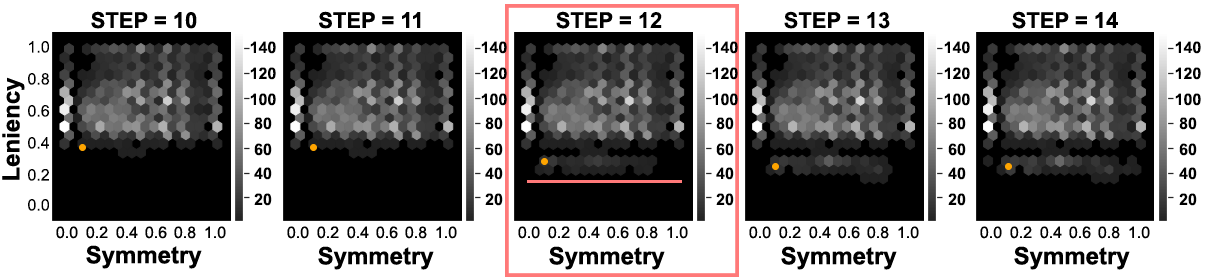
\includegraphics[width=0.8\textwidth]{figures/exp1-lowlen-exploring_new_area/accumulative__X-sym-Y-len-simplified-2.png}}
%\centerline{\includegraphics[width=0.55\textwidth]{figures/low-len/accu__X-sym-Y-len.png}}
\caption{Aggregated TERA using Sym and Len following the low leniency scenario (fig.~\ref{figs:roomsexperiments}.a). Highlights how the design introduces new generative region to the algorithm. In red (step 12) it is highlighted when the design enters a new region of the space and MAP-Elites is then able to generate individuals in that region, explained in detail in Case 1.}
\label{figs:exp1}
\end{figure*}

We have conducted a series of experiments on EDD to analyze the \emph{adaptability} and \emph{stability} of IC MAP-Elites, as well as the effects of the interaction for MAP-Elites and the user. \emph{Stability} relates to the steady generation of high-performing individuals, while gradually growing the search and stably covering the generative space at each edit step. \emph{Adaptability} relates to the ability of the search to adapt to changing conditions, adjusting the search to the new goals, while still generating high-performing individuals. Both features, relate to the notions of evolvability~\cite{p9doncieux2020-noveltyEvolvability}, the ability of the search to generate creative individuals in problems with changing conditions.

% as how the search process benefits from the continuous mixed-initiative approach. 

We recorded three different design sessions, called scenarios, where we manually designed, step by step, dungeon rooms with specific target design goals. They are shown in Figure~\ref{figs:roomsexperiments}: a) a boss room - identified as a \textbf{low leniency} design goal; b) a linear room with specific paths and targets - identified as a \textbf{high linearity} design goal, and finally, c) a room where each chamber within is usable - identified as a \textbf{high meso-pattern} design goal. We chose these design goals as they represent key metrics with clear distinct representative goals and design styles that one might create in a dungeon.

% (Figure~\ref{figs:roomsexperiments}): a) low leniency, b) high linearity, and c) high meso-pattern level. 

% , e.g., (a) a final boss room, (b) a linear room with specific paths and targets, and (c) a room where each chamber within is usable; all 3 named in relation to their “associated” dimension. The goals relate to the dimensions because dimensions are orthogonal to some extent to the fitness function in MAP-Elites, which in the case of the dimensions in EDD, make them closer to properties you would aim for when creating levels .e.g., leniency or linearity. Each edition is included as-is in the population and used as a target in the fitness function by IC MAP-Elites, updating corridor, chamber, and inventorial ratios affecting the quality of micro and meso patterns. 

%  Each scenario was run under every combination of EDD's feature-dimensions in pairs ($21$), where the dimensions are
The experiments consist on running these pre-recorded scenarios separately on EDD, step by step with a lapse of $100$ evolutionary generations between steps. Each scenario implies 21 evolutionary runs, one per each pair of feature-dimension, where the dimensions are (table~\ref{tab:dimensions}): leniency (len), linearity (lin), spatial patterns (spa), meso-patterns (meso), symmetry (sym), similarity (sim), and inner similarity (IS). Each edition (i.e., design step) is included as-is in the population and used as a target in the fitness function by IC MAP-Elites, updating corridor, chamber, and inventorial ratios affecting the quality of micro and meso patterns. Every $100$ generations we collect the novel generated individuals to later analyze how the search and the fitness landscape vary after each design step. Step after step, we measure how the explored generative space grows, as well as how distribution and concentration of elites together with the manually edited room traverse the generative space.%, while keeping track of all individuals' fitness scores. 

% (i.e., if the algorithm generates an individual previously generated, we do not 


In all the experiments, the initial population was set to $1000$ mutated individuals. All cells were set to a maximum capacity of $25$ individuals each. In every generation, we selected $5$ cells random, and $5$ parents per cell through tournament selection. The random selection followed a uniform distribution. Offspring were produced through a two-point crossover and a $30$\% mutation chance. Using this setup, between $150$ to $2001$ individuals were produced every $100$ generations, with an average of $373$ unique individuals generated every $100$ generations throughout all runs.

\subsubsection{Metrics}

All our experiments are evaluated and analyzed following the same procedure and metrics, focusing in the novel generated individuals. In particular, we calculated the \textit{coverage} ($\Diamond$), the \textit{average coverage per step} ($\dagger$), and \textit{average fitness} ($\bigcirc$). \textit{Coverage} relates to the percentage of space covered by the search in total and is calculated as the cumulative amount of covered hexagons at the final step divided by the maximum amount in our experiments. \textit{Average coverage} relates to the average coverage per step, i.e., how much of the space is covered at each design step in average, calculated as the cumulative coverage per step divided by the amount of design editions. Finally, \textit{average fitness} calculates the average individual fitness in the search throughout all generations.



% the \textit{cumulative coverage average among all design steps} .

\begin{figure*}[t!]
\centerline{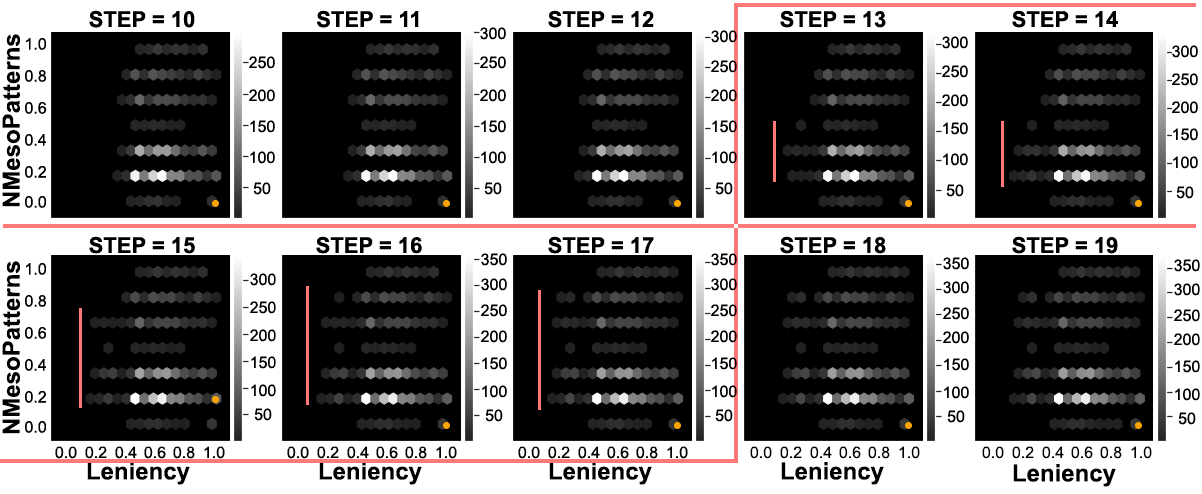
\includegraphics[width=0.8\textwidth]{figures/exp2-highlin-exploringchamber/accumulative__X-len-Y-mesoPat-simplify-2.png}}
%\centerline{\includegraphics[width=0.55\textwidth]{figures/low-len/accu__X-sym-Y-len.png}}
\caption{Aggregated TERA using Len and Meso following the high linearity scenario (fig.~\ref{figs:roomsexperiments}.b). Highlights subtle discovery of new generative regions.  In red (step 12), this subtle discovery is highlighted, explained in detail in Case 2.}
\label{figs:exp2}
\end{figure*}

\subsection{Results and Analysis}

% - Table 2 is included to both serve as a guide for the reader to assess the multiple evaluations done per scenario, and to show the algorithms stability to cover the space while encountering high-performing individuals (QD-properties); thus, the algorithm adapts to the new editions which change the fitness landscape. The first column shows the algorithm’s coverage supported by the second column, which shows that in average MAP-Elites keep exploring and generating novel levels and is not just sporadically generating novel levels. The last column presents the average final fitness by summing the novel levels’ fitnesses after every step (100 generations). Short confidence intervals show that the average numbers do not rely on outliers and that the averages show stable behaviors. Further, table 2 shows an extract of all the pair of dimensions, focusing on the ones that showed the lowest or highest values, which is why all the 21 pair of dimensions are not shown. In retrospect, we can see that the information about the table and why is needed should be extended in the paper, which we will extend with a more precise argumentation for its need in the camera-ready version.

Table \ref{tab:resultsTable} shows an extract of all test results. The results were filtered to only show the pair of dimensions with the lowest or highest values in different metrics. This means that some pair of dimensions are not shown since all their metric values were in between lower and higher scores. Each subtable represents one of the three design scenarios, each of them displaying the metrics described above. The higher and lower scores per column are highlighted in bold and with $\star$, respectively. Confidence intervals are shown per value when using averages. In general, table~\ref{tab:resultsTable} shows IC MAP-Elites' stability to cover the space while encountering high-performing individuals; thus, it is able to adapt to the new editios which change the fitness landscape. Coverage ($\Diamond$), supported by average coverage per step ($\dagger$) and average fitness ($\bigcirc$), shows that in average the algorithm keeps exploring and generating novel and high-performing individuals rather than sporadically generating them.

% Total space coverage ($\Diamond$) is calculated as the cumulative amount of covered hexagons at the final step divided by the maximum amount in our experiments. Average of explored space among all design steps ($\dagger$) is the cumulative amount of covered hexagons divided by the amount of design editions. 

% Table \ref{tab:resultsTable} shows a compilation of all test results. The wider columns represent one of the three design scenarios, each of them displaying the following metrics: $\Diamond$, total space coverage ($\%$); $\dagger$, average $\%$ of explored space among all design steps; $\bigcirc$, average fitness throughout all generations. The higher and lower scores per column are highlighted in bold and with $\star$, respectively. Confidence intervals are shown per value when using averages. Total space coverage ($\Diamond$) is calculated as the cumulative amount of covered hexagons at the final step divided by the maximum amount in our experiments. Average of explored space among all design steps ($\dagger$) is the cumulative amount of covered hexagons divided by the amount of design editions. 


The symmetry and spatial pattern (Sym-Spa) dimension pair explore and cover on average more of the space across all scenarios than others ($\Diamond$). In general, when using either \textit{sym} or \textit{spa}, MAP-Elites is pressured to generate content that maximizes the utility of walls since both use walls as a core building block. Similarly, \textit{Meso} and \textit{IS} are two other dimensions that perform well with others, especially~\textit{Meso}. However,~\textit{Meso} requires combination of shapes with walls and correct placement of tiles; thus, in principle involving more complex operations to achieve high dimensional values. % On the other hand, linearity and spatial pattern (Lin-Spa) explores the least. Linearity does not achieve great results in space exploration, except when linearity is the target design goal (case three) or combined with some other more explorative dimension.

 
% The meso- and spatial pattern (Meso-Spa) dimension pair scores the largest explored space ($\Diamond$) in all scenarios, whereas linearity and spatial pattern (Lin-Spa) explores the least in 3 out of 4. Large explored spaces signify that the good synergy between both dimensions enables the underlying evolutionary algorithm to explore most of it. Meso- and spatial pattern align well with each other, since proper placement of spatial patterns is often favorable to the arrangement of meso-patterns. Linearity does not generally (all dimension pairs including Lin) achieve great results in space exploration, except for the third scenario, where linearity is the target design goal. Combinations involving similarity (Sim) explore less the generative space, but this feature implies searching for individuals that are different-yet-close to the manually edited room, therefore the evolutionary process focuses in areas of the generative space around it.

Overall the average population fitness ($\bigcirc$) is very high with 0.915 in average (of a maximum 1.0) with a narrow confidence interval $\pm$0.01. Symmetry and leniency (Sym-Len) scored the highest in all scenarios while Similarity and Linearity (Sim-Lin) scored the lowest. This shows a stable behavior in the IC MAP-Elites as that the average quality of individuals is high even when large portions of the generative space are explored (high diversity), and regardless of the dimension pair chosen. 

% Notice that the average population fitness ($\bigcirc$) is overall very high, with symmetry and leniency (Sym-Len) scoring the highest in all scenarios. This is very relevant, since it shows a stable behaviour in the IC MAP-Elites as that the average quality of individuals is high even when large portions of the generative space are explored (high diversity), and regardless of the dimension pair chosen. 

IC MAP-Elites works in constant interaction with the edited design. Each step reshapes the fitness landscape to a certain extent, which could hinder the evolutionary process. However, per step, an avg. of 27.34\% of the space is covered by generating novel individuals (i.e., not encountered previously in the population). This, coupled with the relatively narrow confidence intervals, means that the search is constantly exploring the space, diversifying and encountering new spaces. However, as it will be exemplified through the cases, the implicit explorative and exploitative mechanisms of MAP-Elites might not be enough to explore new regions, which can be introduced interactively to MAP-Elites.

%Furthermore, the searched space continuously grows after every step ($\bigtriangleup$). The wider confidence interval is due to the big steps performed at earlier generations, which is expected to some extent by MAP-Elites as there is high-pressure to fill the bins with elites. As more elites are encountered, the lesser bins will remain empty; thus, the search will cover similar spaces, which is what can be observed in most of our experiments. Fontaine et al.~\cite{p9Fontaine2019-hearhstoneDecks} explored and evaluated a similar scenario with good results using MAP-Elites with Sliding Boundaries. In our experiments, When using \textit{Inner Similarity (IS)}, the search grew the most on average regardless of the second dimension, as well as with \textit{Similarity (Sim)}. \textit{Sim} focuses on aesthetical similarity and \textit{IS} internal similarity regarding sparsity and density of tiles. Thus, this could be due to the dimensions pressuring the search to generate different-yet-close individuals to the target room.

% As more elites are encountered, the lesser bins remain empty 

% IC MAP-Elites works in constant interaction with the human designer. Each step reshapes the fitness landscape to a certain extent, which could hinder the evolutionary process. Nevertheless, the searched space continuously grows after every step ($\bigtriangleup$), showing high levels of adaptability to the designer's choices. The linearity and meso-pattern (Lin-Meso) combination shows the higher average explored space per step ($\dagger$) scores in all scenarios. Despite not covering the vastest spaces, individuals are widespread up to almost half the entire space at every step.

%  The dimensions in the ERAs are the same as the IC MAP-Elites, which means that the ERA is effectively the expressivity of the MAP-Elites grid.
The following cases examine TERAs following the different scenarios presented in figure~\ref{figs:roomsexperiments}. Different cases will use either an aggregated TERA step by step or a non-aggregated version showing each step's specific scores in the evaluated dimensions. Each figure's caption and respective case will indicate what type of TERA is used. Non-Aggregated TERAs show the delta maps in the search, meaning where the search has focused and the space covered for a specific step. On the other hand, aggregated TERAs show the density of generated individuals over all steps and the coverage up to the specific step. In each TERA, we also show as an orange dot where the current design is in relation to the used and tested dimensions. Case 1 and 2 examine aggregated TERAs, while case 3 examines non-agreggated TERAs.

% The following cases examine TERAs following the different scenarios presented in figure~\ref{figs:roomsexperiments}. Different cases will use either an aggregated TERA step by step or a non-aggregated version showing each step's specific scores in the evaluated dimensions. Each figure's caption and respective case will indicate what type of TERA is used. Non-Aggregated TERAs show the delta maps in the search, meaning where the search has focused and the space covered for a specific step. On the other hand, aggregated TERAs show the density over all steps of the generated individuals and the covered space up to the specific step. In each TERA, we also show as an orange dot where the current design is in relation to the used and tested dimensions. Case 1 and 2 examine aggregated TERAs, while case 3 examines non-agreggated TERAs.

%The following cases examine ERAs following the different scenarios presented in figure~\ref{figs:roomsexperiments}. Case 1 and 2, examine ERAs where each step is subsequently aggregated, while case 3 and 4, examine ERAs where each step are the unique individuals generated at each step. 

%non-aggregated ERAs are indeed delta maps showing differences. Specifically, they show where the search has focus and the covered space on the current step. On the other hand, aggregated ERAs show more general information of the expressive range, such as the whole generated space and the density of the generated levels.

% \begin{figure*}[t!]
%     \centering
%     \subfloat[Aggregated TERA using Sym and Len following the low leniency scenario (fig.~\ref{figs:roomsexperiments}.a). Highlights how the design introduces new generative area to the algorithm. In red (step 12) it is highlighted when the design enters a new area of the space and MAP-Elites is then able to generate individuals in that area, explained in detail in Case 1.\label{fig:go}]{%
%       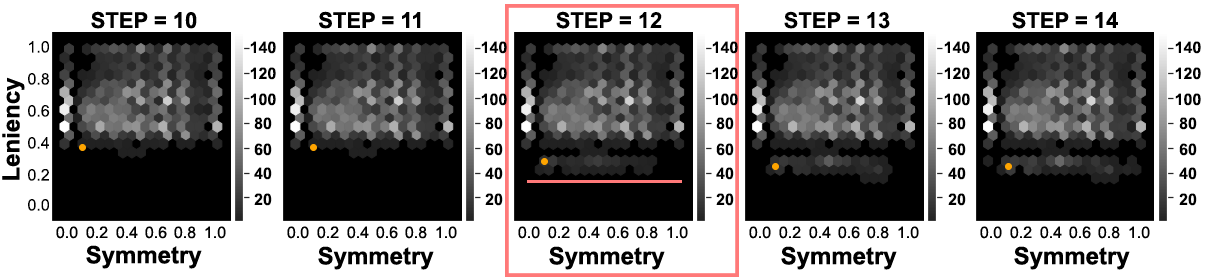
\includegraphics[width=0.8\textwidth]{figures/exp1-lowlen-exploring_new_area/accumulative__X-sym-Y-len-simplified-2.png}
%      }\hfill
%      \subfloat[Aggregated TERA using Len and Meso following the high linearity scenario (fig.~\ref{figs:roomsexperiments}.b). Highlights subtle discovery of new generative areas.  In red (step 12), this subtle discovery is highlighted, explained in detail in Case 2.\label{fig:go}]{%
%       \includegraphics[width=0.8\textwidth]{figures/exp2-highlin-exploringchamber/accumulative__X-len-Y-mesoPat-simplify.png}
%      }\hfill
%     %  \medskip
%      \subfloat[Non-aggregated TERA using Sym and Meso following the high meso-pattern level scenario (fig.~\ref{figs:roomsexperiments}.c). Highlights overall properties of interacting with MAP-Elites. Lighter areas identified with a, b, c, and d, represent the main areas of focus explained in detail in Case 3.\label{fig:scf}]{%
%       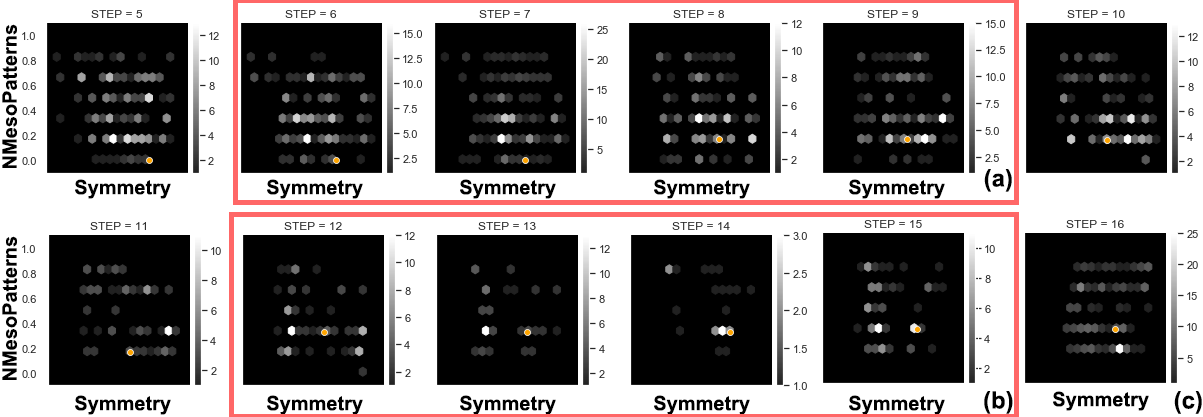
\includegraphics[width=0.8\textwidth]{figures/exp4-mesopat-explorDeadend_leavesearch/simple__X-sym-Y-mesoPat-simplify-combo.png}
%      }
    
%     \caption{Example archetypical paths from different frequent sequences.}
%     \label{fig:archetypical-examples}
% \end{figure*}







\begin{figure*}[ht]
\centerline{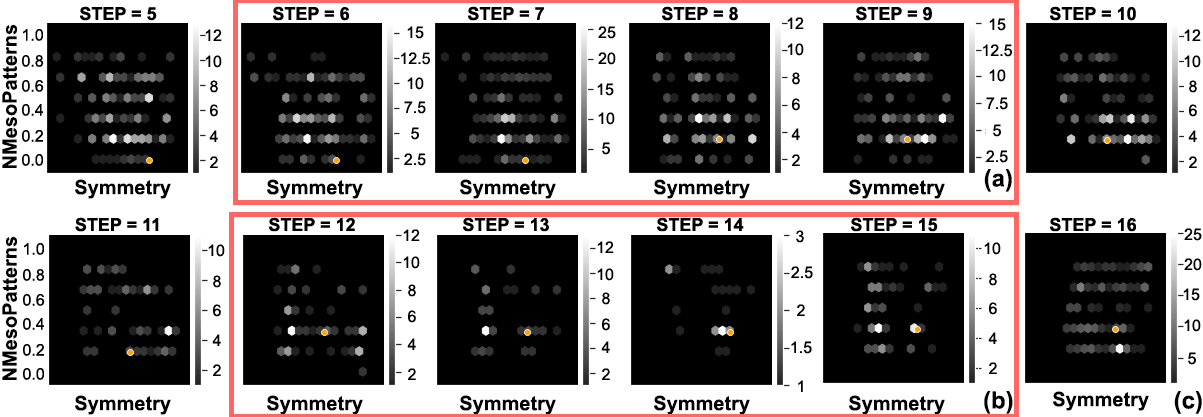
\includegraphics[width=0.8\textwidth]{figures/exp4-mesopat-explorDeadend_leavesearch/simple__X-sym-Y-mesoPat-simplify-combo-2.png}}
%\centerline{\includegraphics[width=0.55\textwidth]{figures/low-len/accu__X-sym-Y-len.png}}
\caption{Non-aggregated TERA using Sym and Meso following the high meso-pattern level scenario (fig.~\ref{figs:roomsexperiments}.c). Highlights overall properties of interacting with MAP-Elites.a, b, and c, represent the main areas of focus explained in detail in Case 3.}
\label{figs:exp3}
\end{figure*}





% \begin{figure*}[t]
% \centerline{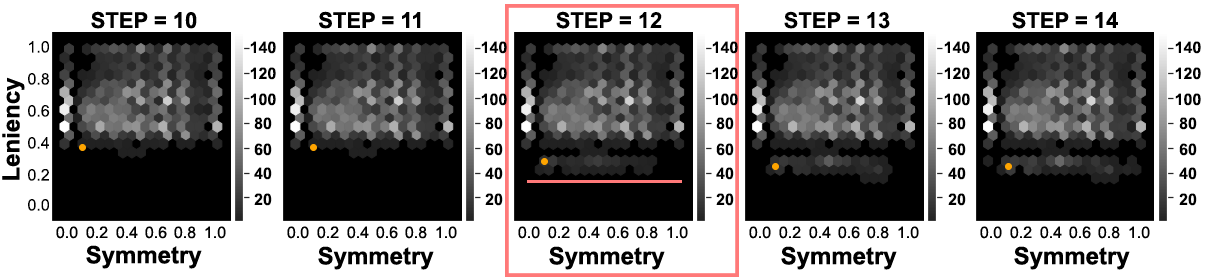
\includegraphics[width=0.8\textwidth]{figures/exp1-lowlen-exploring_new_area/accumulative__X-sym-Y-len-simplified-2.png}}
% %\centerline{\includegraphics[width=0.55\textwidth]{figures/low-len/accu__X-sym-Y-len.png}}
% \caption{Aggregated TERA using Sym and Len following the low leniency scenario (fig.~\ref{figs:roomsexperiments}.a). Highlights how the design introduces new generative area to the algorithm. In red (step 12) it is highlighted when the design enters a new area of the space and MAP-Elites is then able to generate individuals in that area, explained in detail in Case 1.}
% \label{figs:exp1}
% \end{figure*}

% \begin{figure}[h]
% \centerline{\includegraphics[width=0.47\textwidth]{figures/exp2-highlin-exploringchamber/accumulative__X-len-Y-mesoPat-simplify.png}}
% %\centerline{\includegraphics[width=0.55\textwidth]{figures/low-len/accu__X-sym-Y-len.png}}
% \caption{Aggregated TERA using Len and Meso following the high linearity scenario (fig.~\ref{figs:roomsexperiments}.b). Highlights subtle discovery of new generative areas.  In red (step 12), this subtle discovery is highlighted, explained in detail in Case 2.}
% \label{figs:exp2}
% \end{figure}


% \begin{figure}[ht]
% \centerline{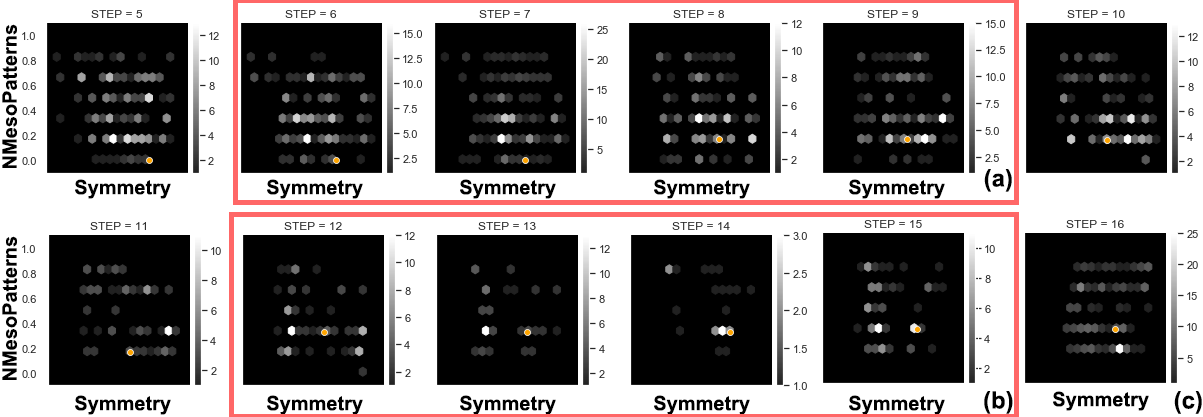
\includegraphics[width=0.47\textwidth]{figures/exp4-mesopat-explorDeadend_leavesearch/simple__X-sym-Y-mesoPat-simplify-combo.png}}
% %\centerline{\includegraphics[width=0.55\textwidth]{figures/low-len/accu__X-sym-Y-len.png}}
% \caption{Non-aggregated TERA using Sym and Meso following the high meso-pattern level scenario (fig.~\ref{figs:roomsexperiments}.c). Highlights overall properties of interacting with MAP-Elites. Lighter areas identified with a, b, c, and d, represent the main areas of focus explained in detail in Case 3.}
% \label{figs:exp3}
% \end{figure}

% \begin{figure*}[t]
%     \centering
%     \begin{subfigure}[t]{0.33\textwidth}
%         \centering
%         \includegraphics[width=0.95\textwidth]{figures/exp5-linearity-Highlen/__X-lin-Y-mesoPat.png}
%         \caption{Linearity-\#MesoPatterns}
%     \end{subfigure}%
%     \begin{subfigure}[t]{0.33\textwidth}
%         \centering
%          \includegraphics[width=0.95\textwidth]{figures/exp5-linearity-Highlen/__X-lin-Y-spaPat.png}
%         \caption{Linearity-\#SpatialPatterns}
%     \end{subfigure}
%     \begin{subfigure}[t]{0.33\textwidth}
%         \centering
%         \includegraphics[width=0.95\textwidth]{figures/exp5-linearity-Highlen/__X-lin-Y-sym.png}
%         \caption{Linearity-Symmetry}
%     \end{subfigure}%
%     \caption{Selected non-Aggregated ERAs using Linearity and following the high leniency scenario (fig.~\ref{figs:roomsexperiments}.a.). The ERAs present pair of dimensions, reusing linearity, where the design remains still for most of the steps in the generative space yet MAP-Elites stably generates novel individuals in a substantial area. Explained in detail in~\ref{sec:case4}.}
%     \label{figs:exp4}
% \end{figure*}

%\subsubsection{Case 1 - Design introducing a new area of the generative space}
\subsubsection{Case 1 - Design Opens New Regions of the Generative Space} \label{sec:case1}

In this case, we analyze the interaction with IC MAP-Elites through examining the generative space when using Sym and Len as dimensions (figure~\ref{figs:exp1}) following the low leniency scenario depicted in figure~\ref{figs:roomsexperiments}.a. The scenario aimed to gradually increase the room's challenge while dividing it into two clear and connected areas.

Table~\ref{tab:resultsTable} shows that this pair of dimensions do not have the best scores except for the $\overline{fitness}$ ($\bigcirc$). This indicates that these dimensions are able to stably find high-performing individuals (above the avg.) while adapting to the new designs exploring an average of 21.54 and a total of 68.1\%. Moreover, in fig~\ref{figs:exp1}, for several steps, half of the generative space is completely unexplored, which could indicate that in those regions, dimensions would be mutually exclusive. 

However, at step 12 (highlighted in red in fig~\ref{figs:exp1}), when reaching a low leniency score, the design enters an unexplored region of the generative space, which subsequently enables IC MAP-Elites to search and generate high-performing individuals in the new region. Furthermore, there is a significant rise in the number of unique individuals generated with a high concentration on the new region, spreading over the already explored space.

\subsubsection{Case 2 - Subtle Changes in the Design Reflected in the Generation of MAP-Elites} \label{sec:case2}

Case 1 showed that by entering an unexplored region of the generative space, the designer could show possibilities for the algorithm and influence the search, yet more subtle guidance is possible. Figure~\ref{figs:exp2} presents such a case. We focus on the high linearity scenario (fig.~\ref{figs:roomsexperiments}.b), where the goal was to create a single narrow corridor between the top and left door and add some objective at the bottom entrance. Through this, we not only aimed at high linearity but also tried to promote other main characteristics such as the open chamber/corridor balance, or the combination of meso-patterns.

Similar to the previous case, in figure~\ref{figs:exp2}, it is shown that for many steps, the search does not explore a big part of the generative space. In this case, the room does not move either in the generative space as the changes are not affecting the dimensions. However, between steps 13 to 17, a new region of the generative space is filled (highlighted in red in fig~\ref{figs:exp2}), which indicates that even if changes in the room do not have a direct influence by moving in the generative space, they still can foster exploration in new regions. These main steps are visible in fig.~\ref{figs:roomsexperiments}.b, subfigure 5, and 6 from the left. Specifically, lower leniency regions are generated once the room is divided into a representative corridor and a big open area with a treasure meso-pattern. These stepping-stones gave the needed “building blocks” to MAP-Elites to cross and mutate until the new generative space was explored. Moreover, similarly to the previous case, the algorithms generates significantly more novel individuals during this time  (around 531 novel individuals), and the search covers 20\% of the space, exploiting the new region, akin to Novelty search behavior~\cite{p9liapis2015-ConstrainedNoveltySearch}.

% (the number of novel individuals there is a significant rise in the number of individuals (\~{}531 novel individuals) and a \~{20}\% search grow, concentrating in the new area, akin novelty search's behavior.

%, which is more possible as atleast one of the dimensions matches the design goal of the room. However when

\subsubsection{Case 3 – Exploring Multiple Properties}
\label{sec:case3}

%In case 3, we focus in the high meso-pattern concentration scenario (fig.~\ref{figs:roomsexperiments}.d), where we subdivided the room into small open chambers with clear objectives in them. Furthermore, in this case we analyze the unique individuals generated step by step rather than in an aggregated fashion using Symmetry and \#MesoPatterns as pair of dimensions. 

In this case, we analyze the TERA of unique individuals generated each step using Sym and Meso as dimension pairs (fig.~\ref{figs:exp3}). We heed to the high meso-pattern level scenario (fig.~\ref{figs:roomsexperiments}.c), where we subdivided the room into small open chambers with clear objectives. Overall, in fig.~\ref{figs:exp3} two aspects stand out; firstly, the generative space is explored more at the early steps, as there are fewer constraints from the edited design. Secondly, the generated individuals seem to follow the path taken by the design in the generative space. Supported by the other cases, this indicates that the design can filter the search and point regions of interest for the IC MAP-Elites. %Furthermore,  this pair of dimensions in the specific scenario, have very high scores analyzing the data in table~\ref{tab:resultsTable} for this pair of dimensions in the specific scenario, 

Moreover, opposite to case 1 and as a consequence of filtering the generative space, when the design leaves low scoring regions, the algorithm rapidly disregards creating individuals in those spaces. For instance, the bottom region after step 7 (fig.~\ref{figs:exp3}.a). Further, as the room is changing but without any type of influence in the searched dimensions e.g., steps 12 to 15 (fig.~\ref{figs:exp3}.b), MAP-Elites has difficulties exploring the space. A similar challenge was discussed by Alvarez et al.~\cite{p9Alvarez2020-ICMAPE}, where their experiments showed that the search got to a plateau after 1000 generations due to the MAP-Elites lacking the incentive to explore. Even if their experiments focused on static environments, this case gives further evidence that minimal changes to the design and lack of influence in the generative space, conditions the exploration of space and the generation of novel individuals. 

Lastly, at step 16 (fig.~\ref{figs:exp3}.c), we encounter a similar situation as with fig.~\ref{figs:exp2};  where a design edition enables the needed “building blocks” for MAP-Elites. In this case, it was triggered by the forming of a dead-end chamber pattern, which enables even more meso-patterns to be used and discovered. Rather than finding a new region of the generative space, this time, the search gets rebooted, and therefore, explores all regions generating novel individuals.
% Lastly, in the last step of the scenario i.e., step 24 (fig.~\ref{figs:exp3}.d), the design enters the highest score in the meso dimension. Thus, helping MAP-Elites to find individuals in a previously unexplored area akin to fig.~\ref{figs:exp1}.

%\subsubsection{Case 4 - Linearity as a stable dimension}
%\label{sec:case4}

%When Linearity is paired with any other dimension, it seems to constantly explore and generate novel individuals. However, compared to other dimensions, Linearity also reveals more difficulty in adapting and producing higher-quality individuals. 

%It can be observed in table~\ref{tab:resultsTable} that the avg. explored space among all steps ($\dagger$) is generally higher than the rest of the combinations and to the average in most of the scenarios. This indicates that when using Linearity, MAP-Elites steadily generates more unique individuals per step, regardless of the second dimension or the design goal, yielding a robust dimension with a stable search. Although, there are second dimensions, which create a better synergy such as meso. However, a good result in ($\dagger$) does not guarantee a vast exploration of the space nor higher quality individuals, if compared with the rest, as noted in table~\ref{tab:resultsTable} ($\Diamond$) and ($\bigcirc$), respectively. 

%In figure~\ref{figs:exp4}, we present three ERAs where Linearity is paired with other dimensions, in order to highlight its overall influence in the solution space coverage. We focus on the high leniency scenario (fig.~\ref{figs:roomsexperiments}.a), where the aim was to create an initial room with a central challenge, and a side path to avoid such a challenge and collecting treasures in the way. However, when using linearity, the ERAs look akin, which is also reflected in the values of table~\ref{tab:resultsTable}.

%Moreover, this case shows the extensive and stable generation that occurs when using linearity, and even if in most cases, the exploitation is focused on the area of the design, it seems to be detrimental for the algorithm. Simply observing the ERAs, this seems to be caused by the design not moving within the generative space. However, this is recurrent when using linearity regardless of the scenario, which suggests that linearity is a more independent dimension. Therefore, linearity, while making the search more robust and stable, generates less-quality individuals and adapts less to the edited design.

%\subsubsection{Case 4 - Linearity as a stable dimension}
%\label{sec:case4}

%In this case, we are interested in presenting another phenomena and a dimension that while constantly exploring and generating novel individuals, does not adapt nor produce as higher quality as other dimensions. Linearity as a dimension, it

%When Linearity is paired with any other dimension, it seems to constantly explore and generate novel individuals. However, compared to other dimensions, Linearity also reveals more difficulty in adapting and producing higher-quality individuals. 
%but with difficulties in adapting and producing higher-quality individuals than other dimensions.
%Linearity is a dimension that, when used together with any other dimension, seems to constantly explore and generate novel individuals but with difficulties in adapting and producing higher-quality individuals as other dimensions. 
%It can be observed in table~\ref{tab:resultsTable} that the avg. explored space among all steps ($\dagger$) is generally higher than the rest of the combinations and to the average in most of the scenarios. This indicates that when using Linearity, MAP-Elites steadily generates more unique individuals per step, regardless of the second dimension or the design goal, yielding a robust dimension with a stable search. Although, there are second dimensions, which create a better synergy such as meso. However, a good result in ($\dagger$) does not guarantee a vast exploration of the space nor higher quality individuals, if compared with the rest, as noted in table~\ref{tab:resultsTable} ($\Diamond$) and ($\bigcirc$), respectively. 

%Unlike the other cases, in figure~\ref{figs:exp4} we present three ERAs where Linearity is represented with other dimensions to highlight a phenomenon when using linearity. We focus on the high leniency scenario (fig.~\ref{figs:roomsexperiments}.a), where the aim was to create a more introductory room with a central challenge, and a side path to avoid such a challenge and collecting treasures in the way. However, when using linearity, the ERAs look very similar, which is also reflected in the values of table~\ref{tab:resultsTable}. 

%In figure~\ref{figs:exp4}, we present three ERAs where Linearity is paired with other dimensions, in order to highlight its overall influence in the solution space coverage. 
%Unlike the other cases, in figure~\ref{figs:exp4} we present three ERAs where Linearity is represented with other dimensions to highlight a phenomenon when using linearity. 
%We focus on the high leniency scenario (fig.~\ref{figs:roomsexperiments}.a), where the aim was to create an initial room with a central challenge, and a side path to avoid such a challenge and collecting treasures in the way. However, when using linearity, the ERAs look akin%very similar
%, which is also reflected in the values of table~\ref{tab:resultsTable}.

%Moreover, this case shows the extensive and stable generation that occurs when using linearity, and even if in most cases, the exploitation is focused on the area of the design, it seems to be detrimental for the algorithm. Simply observing the ERAs, this seems to be caused by the design not moving within the generative space. However, this is recurrent when using linearity regardless of the scenario, which suggests that linearity is a more independent dimension. Therefore, linearity, while making the search more robust and stable, generates less-quality individuals and adapts less to the edited design.

% \begin{table*}[t]
% \centering
% \caption{I am thinking on having a table were we have all the dimensions and show some percentages on how they "do" in all the different scenarios. For instance, show the percentage of filled space (how much the pair odf dimensions cover the generative space). Another could be to have the average of covered space in all steps }\smallskip
% \begin{tabular}{lcccccccccccccccc}
% Dimensions & a & a & a & a & a & a & a & a & a & a & a & a & a & a & a & a\\ \hline
% a & a & a & a & a & a & a & a & a & a & a & a & a & a & a & a & a\\ \hline
% \end{tabular}
% %}
% \label{table1}
% \end{table*}

% \begin{table*}[t]
% \centering
% \caption{I am thinking on having a table were we have all the dimensions and show some percentages on how they "do" in all the different scenarios. For instance, show the percentage of filled space (how much the pair odf dimensions cover the generative space). Another could be to have the average of covered space in all steps }\smallskip
% \label{tab:resultsTable}
% \renewcommand\arraystretch{1.2}
% \resizebox{\textwidth}{!}{%
% \begin{tabular}{lcccccccccccccccc}
% \hline
% \multicolumn{1}{|l|}{Dimensions} & \multicolumn{4}{c|}{high len} & \multicolumn{4}{c|}{low len} & \multicolumn{4}{c|}{high lin} & \multicolumn{4}{c|}{meso pat} & \multicolumn{4}{c|}{low lin} & \multicolumn{4}{c|}{spat pat} & \multicolumn{4}{c|}{high sym} & \multicolumn{4}{c|}{nylow len} \\ \hline

% \multicolumn{1}{l|}{} & \multicolumn{1}{c|}{$\Diamond$} & \multicolumn{1}{c|}{$\bigtriangleup$} & \multicolumn{1}{c|}{$\box$} & \multicolumn{1}{c|}{$\bigcirc$} & \multicolumn{1}{c|}{$\Diamond$} & \multicolumn{1}{c|}{$\bigtriangleup$} & \multicolumn{1}{c|}{$\box$} & \multicolumn{1}{c|}{$\bigcirc$} & \multicolumn{1}{c|}{$\Diamond$} & \multicolumn{1}{c|}{$\bigtriangleup$} & \multicolumn{1}{c|}{$\box$} & \multicolumn{1}{c|}{$\bigcirc$} & \multicolumn{1}{c|}{$\Diamond$} & \multicolumn{1}{c|}{$\bigtriangleup$} & \multicolumn{1}{c|}{$\box$} & \multicolumn{1}{c|}{$\bigcirc$} & \multicolumn{1}{c|}{$\Diamond$} & \multicolumn{1}{c|}{$\bigtriangleup$} & \multicolumn{1}{c|}{$\box$} & \multicolumn{1}{c|}{$\bigcirc$} & \multicolumn{1}{c|}{$\Diamond$} & \multicolumn{1}{c|}{$\bigtriangleup$} & \multicolumn{1}{c|}{$\box$} & \multicolumn{1}{c|}{$\bigcirc$} & \multicolumn{1}{c|}{$\Diamond$} & \multicolumn{1}{c|}{$\bigtriangleup$} & \multicolumn{1}{c|}{$\box$} & \multicolumn{1}{c|}{$\bigcirc$} & \multicolumn{1}{c|}{$\Diamond$} & \multicolumn{1}{c|}{$\bigtriangleup$} & \multicolumn{1}{c|}{$\box$} & \multicolumn{1}{c|}{$\bigcirc$} \\ \hline


% % & \multicolumn{1}{c|}{b} & \multicolumn{1}{c|}{b} & \multicolumn{1}{c|}{b} & \multicolumn{1}{c|}{b} & \multicolumn{1}{c|}{b} & \multicolumn{1}{c|}{b} & \multicolumn{1}{c|}{b} & \multicolumn{1}{c|}{b} & \multicolumn{1}{c|}{b} & \multicolumn{1}{c|}{b} & \multicolumn{1}{c|}{b} & \multicolumn{1}{c|}{b} & \multicolumn{1}{c|}{b} & \multicolumn{1}{c|}{b} \\ \hline

% \multicolumn{1}{|c|}{Len-Lin} & 62.5\% & 62.5\% & 62.5\% & \multicolumn{1}{c|}{50\%} & 62.5\% & 62.5\% & 62.5\% & \multicolumn{1}{c|}{50\%} & 62.5\% & 62.5\% & 62.5\% & \multicolumn{1}{c|}{50\%} & 62.5\% & 62.5\% & 62.5\% & \multicolumn{1}{c|}{50\%} & 62.5\% & 62.5\% & 62.5\% & \multicolumn{1}{c|}{50\%} & 62.5\% & 62.5\% & 62.5\% & \multicolumn{1}{c|}{50\%} & 62.5\% & 62.5\% & 62.5\% & \multicolumn{1}{c|}{50\%} & 62.5\% & 62.5\% & 62.5\% & \multicolumn{1}{c|}{50\%} \\ \hline

% \multicolumn{17}{l}{$\Diamond$ Total space searched till last design step\ \
% $\bigtriangleup$ Average space searched among all the design steps}
% \end{tabular}%
% }
% \end{table*}
\subsection{Discussion}

% Results from Case 1 indicates that areas that 

% Results from Case 1 indicate that formerly unreached areas in the generative space, due to seemingly mutually exclusive dimension scores, are explored after the design enters such area and we add the example in the population. This helps the algorithm to generate new individuals and fosters the search for novel individuals. Case 3 also shows how the algorithm can drive the search and generation by moving across the generative space with simple edits. In turn, the algorithm focuses on exploiting areas closely related to the design. In practice, by understanding this dynamic, we could identify where the designer is in the generative space and then either foster the selection of cells farther away to exploit a larger area or focus around the design to provide perhaps more relevant suggestions.

% Results from Case 1 indicate that formerly unreached areas in the generative space, due to seemingly mutually exclusive dimension scores, can be explored after manually inputting an example in the unreached area. This helps the algorithm to generate new individuals and fosters the search for novel individuals. However, the opposite result can also occur, as exemplified in Case 3, where the design moves away from certain areas in the generative space, and the IC MAP-Elites quickly stops producing individuals in those spaces.

% In Case 2 and 3, the exploration of new areas and the generation of novel individuals are fostered once the room is more structured. In Case 3,

% In Case 2 and 3, the exploration of new areas in the generative space and the generation of novel individuals in previously explored spaces are fostered once that the room is structured and some dead-ends appear. Case 3 also shows how the algorithm can drive the search and generation by moving across the generative space with simple edits. In turn, the algorithm focuses on exploiting areas closely related to the design. In practice, by understanding this dynamic, we could identify where the designer is in the generative space and then either foster the selection of cells farther away to exploit a larger area or focus around the design to provide perhaps more relevant suggestions. Nevertheless, adapting to the design path in the generative space can carry negative consequences. 

Our evaluation shows that IC MAP-Elites has a high degree of adaptability to dynamic environments, adapting the generated content to the design process and design goals while stably generating high-performing and diverse solutions. For MI-CC systems and interactive approaches as in EDD, this is especially relevant and important. The fitness function adapts to the current design; thus, adaptability and stability go hand in hand. Furthermore, the deployment of an MI-CC approach in a scenario as the ones presented would benefit both Map-Elites and the human designer. On the one hand, it enables MAP-Elites to explore more of the generative space while producing quality solutions. On the other hand, users would have more control over the suggestions as they seamlessly influence and guide the search and generation with their design, in a similar approach to Anderson et al., who explored explicit human guidance in the automated solution search~\cite{p9anderson2000-humanguidedSearch}. 

% explores human-AI collaboration by introducing explicit human guidance in the automated solution search~\cite{p9anderson2000-humanguidedSearch}, which was further expanded and elaborated as Interactive Evolution by Takagi~\cite{p9Takagi2001-InteractiveEvo}.~\cite{p9anderson2000-humanguidedSearch}.

We also observe that when using Linearity as a dimension, IC MAP-Elites performed quite stably in all our scenarios regardless of the design traversing around the generative space or not, which indicates that Linearity is more robust and stable and more agnostic and independent from the design. These characteristics are beneficial in certain cases, but based on the results presented in table~\ref{tab:resultsTable}, this stability comes at the expense of adaptability and higher fitness scores.

Furthermore, Alvarez et al.~\cite{p9Alvarez2020-ICMAPE} presented an analysis of IC MAP-Elites in a static scenario, where on average the covered space of MAP-Elites after $5000$ generation was 52.4\% using pair of dimensions and 51.7\% using all seven dimensions. Our results show a clear advantage for MAP-Elites when used continuously and interactively with an avg. coverage of 70.9\%. However, when the design remains still in the space defined by the dimensions, exploration is hindered; thus, what dimensions are used and how the design maps to them is crucial.

% However, Alvarez et al.~\cite{p9Alvarez2020-ICMAPE} use a similar experiment set up, executing MAP-Elites for 5000 generations in a static environment resulting in limited coverage, which we expect to achieve 

% Disabling adaptation mechanisms would effectively render the algorithm static and in this case make the algorithm agnostic to any edition, which could further support the findings in this paper. In [1] (discussed in the paper), the authors’ experiments use a similar set up, executing IC MAP-Elites for 5000 generations in a static environments. Their results showed constant unexplored areas with 52.4of coverage in average, which as we discuss in our paper, when adapting to changes we increase the average to 70.9. We expect to encounter similar results if disabling adaptive mechanism as the approach would be even more static and agnostic than [1]. Likewise, in [1] they also conduct the experiment using an objective-based GA, which we also expect to encounter similar results. Since we are given 1 extra page, we will add a discussion over this and add it as an interesting future work avenue, as we think that this information is beneficial and could be used to further evidence the benefits of interaction.

Finally, we used and introduced TERAs to analyze the dynamic behaviors in generative systems and algorithms, and observe the effects of changes over time in the expressive range based on the edition steps. We used two variations, non-aggregated TERA, which shows the delta maps of the search, and aggregated TERA, showing the search density and aggregated results. TERAs are generic and could be used with other generative system to evaluate their dynamics by simply defining a pair of features and a step period such as design editions, amount of generations, or whenever a suggestion is applied. TERAs can also be used to spot key and non-trivial steps or changes that have an effect in the search, which can help to understand more in-depth the sensibility of the algorithm and the system. 

% Our evaluation shows that IC MAP-Elites has a high degree of adaptability to dynamic environments, adapting the generated content to the design process and design goals while stably generating high-performing and diverse solutions. This is made possible due to the inherent properties of QD-algorithms. For MI-CC systems and interactive approaches as in EDD, this is especially relevant and important. The fitness function adapts to the current design; thus, adaptability and stability go hand in hand. Furthermore, the deployment of an MI-CC approach in a scenario such as the ones presented would benefit both Map-Elites and the human designer. On the one hand, it enables MAP-Elites to explore more of the generative space while producing quality solutions; on the other hand, users would have more control over the suggestions as they influence and guide the search and generation.


% \subsubsection{How to use the findings in this paper?}

% Here we should describe how other interactive tools can use the findings in this paper, the impact of the presented dynamics (borrow what was the final conclusion)

% IC MAP-Elites shows a high degree of adaptability to dynamic environments, adapting the generated content to the design process and design goals while stably generating high-performing and diverse solutions. This is made possible due to the inherent properties of QD-algorithms. For MI-CC systems and interactive approaches as in EDD, this is especially relevant and important. The fitness function adapts to the current design; thus, adaptability and stability go hand in hand. Furthermore, the deployment of an MI-CC approach in a scenario such as the ones presented would benefit both Map-Elites and the human designer. On the one hand, it enables MAP-Elites to explore more of the generative space while producing quality solutions; on the other hand, users would have more control over the suggestions as they influence and guide the search and generation.



% An interesting future project would be to evaluate and compare 

% Using a similar methodology as the one presented in this paper, an interesting project for future work would be to evaluate and compare MAP-Elites and its properties to other co-creative systems using different algorithms such as reinforcement learning~\cite{p9delarosa2020-RLbrushMixedinit,guzdial-lvldsg-aiide-2018} or constraint solving algorithms~\cite{p9Karth2019-pcgmlDiscriminativeLearning}.
\subsection{Conclusions and Future Work}

% \begin{itemize}
%     \item ADD ABOUT FUTURE WORK ON EVALUATING THIS WITH A NON-INTERACTIVE VERSION AND USING OTHER ALGORITHMS. 
%     \item important to point out that static evaluation was done in~\citepninth{p9Alvarez2020-ICMAPE}
% \end{itemize}

This paper analyzes and evaluates the benefits of dynamically interacting with quality-diversity algorithms, specifically, the IC MAP-Elites. We have examined the adaptability and stability of MAP-Elites in relation to 21 dimension pairs highlighting different characteristics and properties through different simulated design scenarios. We examined key metrics when exploring the generative space, as depicted in table~\ref{tab:resultsTable}, and conducted three different case studies that highlighted different dynamics with the algorithm.
% IC MAP-Elites shows a high degree of adaptability to dynamic environments, adapting the generated content to the design process and design goals while stably generating high-performing and diverse solutions. This is made possible due to the inherent properties of QD-algorithms. For MI-CC systems and interactive approaches as in EDD, this is especially relevant and important. The fitness function adapts to the current design; thus, adaptability and stability go hand in hand. Furthermore, the deployment of an MI-CC approach in a scenario such as the ones presented would benefit both Map-Elites and the human designer. On the one hand, it enables MAP-Elites to explore more of the generative space while producing quality solutions; on the other hand, users would have more control over the suggestions as they influence and guide the search and generation.

% While our results show several MAP-Elites’ properties and promising ways to improve the MI-CC workflow, further evaluation is needed with human users to assess these properties in-the-wild and evaluate the interactive dynamic between humans and algorithms. To further highlight the importance of interaction, it would be interesting to analyze and compare with MAP-Elites disabling adaptive mechanisms (i.e., rendering the algorithm static and agnostic to changes) and with other non QD algorithms. Likewise, another interesting project for future work, would be to evaluate and compare IC MAP-Elites using TERAs with other co-creative systems using different algorithms such as reinforcement learning~\citepninth{p9delarosa2020-RLbrushMixedinit,guzdial-lvldsg-aiide-2018} or constraint solving algorithms~\citepninth{p9Karth2019-pcgmlDiscriminativeLearning}.
 
While our results show several MAP-Elites’ properties and promising ways to improve the MI-CC workflow, further evaluation is needed with human users to assess these properties in-the-wild and evaluate the interactive dynamic between humans and algorithms. To further highlight the importance of interaction, it would be interesting to analyze and compare with MAP-Elites disabling adaptive mechanisms (i.e., rendering the algorithm static and agnostic to changes) and with other non QD algorithms. Likewise, another interesting project for future work, would be to use TERAs to compare IC MAP-Elites with other co-creative systems using other algorithms such as reinforcement learning~\citepninth{p9delarosa2020-RLbrushMixedinit,p9guzdial-lvldsg-aiide-2018} or constraint solving algorithms~\citepninth{p9Karth2019-pcgmlDiscriminativeLearning}.
 
% Using a similar methodology as the one presented in this paper, an interesting project for future work would be to evaluate and compare MAP-Elites and its properties to other co-creative systems using different algorithms such as reinforcement learning~\citepninth{p9delarosa2020-RLbrushMixedinit,guzdial-lvldsg-aiide-2018} or constraint solving algorithms~\citepninth{p9Karth2019-pcgmlDiscriminativeLearning}.


%In this paper, we also present a methodology that extends, to some extent, the work by Smith and Whitehead~\citepninth{p9Smith:2010:Expressive-range} to continuously evaluate generative systems using simulated design sessions and aggregated and non-aggregated ERAs, which highlights properties and dynamics of the algorithms. Thus, an interesting future work would be to use such an approach to evaluate and compare MAP-Elites and its properties to other co-creative systems using different algorithms such as reinforcement learning~\citepninth{p9delarosa2020-RLbrushMixedinit,guzdial-lvldsg-aiide-2018} or constraint solving algorithms~\citepninth{p9Karth2019-pcgmlDiscriminativeLearning}.

%Similarity and Inner Similarity were excluded from the results given that these two dimensions change dynamically as the design changes. Preliminary observations from table~\ref{tab:resultsTable}, indicates that when using IS the generative space is very much covered while retaining an overall high fitness. This points towards a robust dimension, highly adaptable, and with stable growth and performance, but at the expense of general stability and reliability in a mixed-initiative setup as it . Analysis of these dynamic dimensions is left for future work. 

Finally, a promising step is to analyze MAP-Elites together with surrogate designer models that capture preference, style, and design processes~\citepninth{p9Liapis2013-designerModel,p9Alvarez2020-DesignerPreference,p9alvarez2020-designerpersonas}, and how these influence the properties discussed in this paper. For instance, Designer Personas~\citepninth{p9alvarez2020-designerpersonas} could be used to explore how the user's design moves through the space, identifying possible paths, and analyzing if changes, i.e., moving between style clusters, connect to key moments in the search.

\bibliographystylepninth{ieeetr}
\bibliographypninth{included-papers-tex/paper-9/references.bib}